\newcommand{\corriger}[1]{\textcolor{red}{#1}}
\chapter{Contexte général} \label{intro} \label{chapitre_1}
\minitoc
	
\clearpage

\section{L'évolution de l'agriculture}

 Les plantes représentent plus de 80~\% de l'alimentation humaine \citep{FAO2017}. 
On estime que seulement quatorze espèces de  plantes cultivées fournissent la majeure partie de la nourriture destinée à la consommation humaine \citep{Strange2005}.
 En particulier, la population mondiale dépend essentiellement des cultures vivrières de base (céréales, légumineuses,  tubercules) \citep{FAO2017}. Outre ces cultures vivrières, d'autres cultures sont importantes dans l'économie de nombreux pays en développement et sont destinées principalement à l'exportation (la banane, la canne à sucre ou encore la tomate).
De ce fait, la production végétale est essentielle à la sécurité alimentaire qui se traduit par le fait que \og tous les êtres humains ont  la possibilité physique, sociale et économique de se procurer une nourriture suffisante, saine et nutritive afin  de satisfaire leurs besoins et préférences alimentaires pour mener une vie saine et active \fg{} \citep{FAO2017}. Assurer cette sécurité alimentaire dans le contexte d'une population mondiale en croissance  est un enjeu difficile, mais incontournable et crucial \citep{Tilman2011}. Les prédictions indiquent que ce défi actuel  nécessite une augmentation de la production agricole d'au moins 50~\% d'ici 2050 \citep{Tilman2011}. 
	
	Les bioagresseurs  aériens et telluriques  (virus, bactéries, oomycètes, champignons, nématodes) et les mauvaises herbes constituent une menace pour la sécurité alimentaire, puisqu'ils peuvent endommager les cultures, réduisant l'accès à la nourriture et causant des répercussions économiques considérables. 
%Les épidémies causées par des agents pathogènes sont une cause majeure de variations annuelles de la production agricole et peuvent même provoquer des famines.
	Par exemple, le mildiou de la pomme de terre est une maladie redoutable provoquée par le champignon \textit{Phytophtora infestans}. Elle frappa l'Europe dans les années 1840 et entraîna  des millions de morts en Irlande à cause de la famine \citep{Large1940, Spielman1991}. 
	%Les principales cultures dans le monde et leurs principales maladies sont très bien répertoriées dans la revue de (strange2005).  

	Depuis l'origine de l'agriculture, la protection des plantes a pour objectif de sécuriser les récoltes des agriculteurs, ainsi que de nourrir les humains et les animaux en  régulant les maladies des plantes \citep{Stukenbrock2008}. 
	Les systèmes de culture traditionnels reposaient avant tout sur les ressources humaines, la force animale et des écosystèmes quasi naturels (forte hétérogénéité  environnementale,  forte diversité des espèces et faible
densité de plantes). Cependant, depuis les années 1960, l'intérêt pour ces types de systèmes  s'est  considérablement réduit à cause des progrès dans le domaine de la chimie  et de la biologie, qui ont permis un changement radical et une intensification des systèmes de culture \citep{Meynard2003}.% Aujourd'hui, l'impact des pesticides et des pratiques culturales sur l'environnement et la santé des agriculteurs et des consommateurs sont de mieux en mieux documentés 
	 %Deuxièmement,  dans un contexte social-économique et environnemental prédéfini, d'un nouveau modèle d'agriculture   plus durable, plus respectueuse de l'environnement qui tend vers une augmentation significative des rendements des cultures.


\subsection{L'agriculture moderne et son impact environnemental et sanitaire}

	 Au milieu du XXème siècle, de nombreux pays d'Europe ont dû rapidement se reconstruire, se réorganiser et moderniser leur agriculture suite à la seconde guerre mondiale. Ces profonds changements nécessitaient avant tout d'augmenter rapidement et efficacement la production agricole pour assurer l'autonomie alimentaire et la relance économique. Dès lors, les pratiques agricoles ont radicalement changé les écosystèmes agricoles et ont permis une expansion démographique de la population mondiale, passant de 2,5 milliard d'habitants (après à la seconde guerre) à 7 milliards  de nos jours   \citep{Gerland2014}. 
	Nous avons assisté en quelques décennies à une augmentation spectaculaire des rendements des cultures et une protection efficace contre les bioagresseurs à travers l'agriculture moderne \citep{FAO2017}. En effet, depuis le début des années 60,  les pratiques agricoles s'accompagnaient de l'utilisation systématique et massive de pesticides chimiques pour lutter contre les bioagresseurs \citep{Pretty2008,Butault2010, Tilman2001}.
La France était en 2011 le troisième consommateur mondial de produits phytosanitaires, derrière les États-Unis et la Chine \citep{Zhang2011}.  
	Par ailleurs, ce modèle reposait également  sur la modernisation du matériel agricole, la fertilisation, l'irrigation et l'amélioration variétale pour permettre d'augmenter les surfaces cultivées et les rendements des cultures \citep{Brisson2010, Grassini2013, Ray2012}.
La monoculture, consistant à cultiver la même variété sur les mêmes parcelles et souvent à grande échelle, a été une pratique largement utilisée par l'agriculture moderne.  En France, les monocultures de  maïs et  blé  couvrent aujourd’hui 8~\% des surfaces assolées \citep{Fuzeau2012}.

	De nos jours, les répercussions de ce modèle agricole sont bien connues.
Les effets nocifs   des produits phytosanitaires sur la santé humaine et sur l’environnement ne sont plus  à démontrer \citep{Tilman2011, Nicolopoulou-stamati2016}.  L’utilisation massive d’engrais chimiques et  de produits phytosanitaires a eu des effets extrêmement néfastes en termes de pollution des écosystèmes d’eau douce, des nappes phréatiques et des sols \citep{Tilman1999, Stoate2001, Moss2008, Tilman2011}.
Des problèmes liés à l'utilisation de ces produits sur  l'eau potable ont aussi été rapportés à  de nombreuses reprises \citep{Tilman1999, Carpenter1998}. En effet, l’azote est l’un des polluants de l’eau le plus observé dans le monde, particulièrement dans les pays développés. La quantité d’engrais azotés utilisée dans le monde a fortement augmenté au cours des  dernières années \citep{Tilman1999} et présente  un risque pour la santé humaine lorsque cette substance  se retrouve dans l'eau.
	Par ailleurs, l'évolution continue et profonde de l'agriculture a conduit à une diminution des espèces cultivées et à des rotations de cultures de plus en plus courtes dans les systèmes maraîchers et dans les grandes cultures \citep{Bennett2012, Zhan2015}. Ce mode d'agriculture moderne en faveur d'un travail du  sol  intensif par la mécanisation  a joué un rôle majeur dans l'appauvrissement des sols  \citep{Matson1997}.
	De récentes études ont rapporté  un déclin très important de la  biodiversité à cause des pratiques agricoles (monocultures, rotations courtes et peu diversifiées) et de l'usage des pesticides  \citep{Ceballos2017, Geiger2010, Potts2010, Seibold2019, Bommarco2013}. %Enfin, l’élevage et la déforestation jouent un rôle majeur dans le changement climatique (responsable de 24~\%
%émissions de gaz à effet de serre, GIEC 2014). Le secteur de l’élevage contribue pour 14,5~\% aux émissions de
%gaz à effet de serre dues aux activités humaines et consomme énormément de ressources finis (FAO).

	En conclusion, ce modèle d’agriculture intensive, du fait de ses répercussions négatives
sur l’environnement, la santé humaine et de sa dépendance à des ressources finies, a atteint ses limites \citep{Tilman2002}. Il paraît donc urgent et important de sortir de ce modèle.
Pourtant, est-il possible de s'en affranchir dans un contexte où nourrir l'importante population mondiale  constitue un objectif incontournable \citep{Movahedi2009} ?   Pour répondre à cette question, nous proposons dans la suite d'identifier certains  leviers  pour répondre à la demande alimentaire et ainsi proposer des solutions plus efficaces en termes de protection des cultures.
	 
%Toutefois, de plus en plus d'animaux sont élevés de manière intensive et nourris avec des céréales et des huiles bon marché et énergétiquement inefficaces. Dans les pays industrialisés, 73~\% des céréales sont destinées uniquement à l'alimentation animale  \citep{Pretty2008}. Par conséquent ce modèle d'intensification dans le secteur de l'élevage est extrêmement utilisateur de ressources naturelles et dommageable pour l'environnement \citep{Stoate2001}.


\subsection{Vers une agriculture plus  durable}
	 
	L'agriculture devra nourrir d'ici 2050 9,7 milliards d'habitants \citep{Gerland2014}. 
Dans ce contexte, trouver des stratégies de protection des cultures efficaces et durables
est devenu un défi majeur.
Cependant,  la production agricole mondiale stagne  voire diminue ces dernières années
pour de nombreuses cultures et
dans différentes régions du monde \citep{Brisson2010, Ray2012,
Grassini2013, Cassman2010}. Ce ralentissement est dû notamment à la diminution progressive
de sols cultivables à travers le monde, à l’appauvrissement de la biodiversité, à l'émergence de ravageurs, d'agents pathogènes et de  maladies des cultures, et  à la raréfaction des ressources naturelles \citep{Cordell2009}. 
Pour répondre à la demande alimentaire, la croissance du  secteur de la production agricole doit être assurée  en tenant compte du nombre limité de surfaces cultivables et en jouant sur deux principaux leviers \citep{Movahedi2009} :
\begin{itemize}[nosep]
\item réduire les risques de perte de production,
\item augmenter très significativement les rendements des récoltes.
\end{itemize}

	Les terres arables couvrent actuellement 1\,550 millions d’hectares dans le
monde \citep{FAO2017}. On estime que  120 millions d’hectares (soit une augmentation de 8~\%) viendront
encore s’y ajouter d’ici 2030, mais par la suite il n'y aura plus d'autres surfaces à exploiter \citep{Movahedi2009}. Cette limite sur les surfaces cultivables est due à trois facteurs. Premièrement, la quantité des sols abandonnés (principalement à cause de la désertification, l'érosion, la salinisation)  n'a de cesse d'augmenter (3,5 millions d’hectares par an) \citep{Movahedi2009}. Deuxièmement, les nouvelles terres potentiellement disponibles  pour l'agriculture sont demandées aussi par  d'autres secteurs d'activités telles que la production de biocarburants et l'urbanisation \citep{Movahedi2009, Tscharntke2012}. Troisièmement, il est important de protéger les terres de bonne qualité  disponibles puisqu'elles constituent des puits de carbone \footnote{puits de carbone : réservoir (naturel ou artificiel) qui absorbe du carbone en circulation dans la biosphère}  parmi les plus importants  et permettent de préserver  l’équilibre climatique et la biodiversité  \citep{Godfray2010}.  
L'accroissement de la productivité agricole pour nourrir la population mondiale devra forcément passer par une augmentation des rendements des cultures sans pour autant augmenter notablement les surfaces cultivables.

	Globalement, les pertes de rendement directement causées par les bioagresseurs  et les mauvaises herbes chaque année sont estimées à 40~\%  \citep{Agrios2005, Madden1995, Oerke1994} malgré la mise en place de diverses mesures de protection (culturales, génétiques, biologiques ou chimiques). On estime  les pertes économiques provoquées par les bioagresseurs à plus de 300 milliards de dollars par an \citep{Oerke1994}. Différents  facteurs  jouent  un rôle important dans les pertes de rendements et  affectent ainsi les rendements agricoles.
	 
Premièrement, le réchauffement climatique accentue les problèmes sociaux-économi\-ques et environnementaux auxquels doit faire face  l'agriculture  \citep{Fischer2005}. En effet, 
on prévoit que ce changement climatique entraîne une hausse des températures moyennes annuelles, des pluies plus irrégulières et plus intenses, des épisodes de froid intenses et courts, des périodes de sécheresse et des  pénuries d'eau \citep*{EEA2016}. Il est donc fortement possible que ces changements s'accompagnent de pertes agricoles sévères,  également à cause  de  l'émergence ou la réémergence de maladies et de ravageurs des cultures \citep{Garrett2011, Anderson2004, Palumbi2001}.% La  limitation des émissions de gaz à effet de serre (CO2 et aussi le méthane) pourrait permettre de diminuer les effets du changement climatique et donc des  risques de pertes de rendement. 
%Dans le domaine de l'agriculture, un changement de production d’origine animale à forte
%consommation d’eau, de terres et de ressources naturelles, au profit d’une production d’origine végétale pour nourrir les humains pourrait diminuer significativement les émissions de gaz à effet de serre  et donc contribuer à la productivité agricole de manière indirecte à long terme  \citep{Springmann2016}.

% Globalement, on estime que les pertes de rendements pour les trois principaux aliments de base de la consommation humaine  (blé, riz et maïs)   se situeraient entre 20 et 50~\% si la température planétaire augmente de 2$^{\circ}$ C   par rapport à l'ère pré-industrielle \citep{Deutsch2018}. Les États-Unis et la Chine qui produisent la plus grande partie du maïs dans le monde sont également parmi les pays qui devraient connaître les plus fortes augmentations des pertes de récoltes liées aux agents pathogènes \citep{Deutsch2018}. 

	Deuxièmement,  le déclin de la diversité végétale a de nombreuses répercussions négatives en particulier sur le fonctionnement des agroécosystèmes. Il a été démontré depuis longtemps que  la diversification des espèces cultivées joue un rôle majeur dans  la réduction de la transmission des maladies par les agents pathogènes par  \og effet de dilution \fg{} \citep{Mundt1994, Mundt2002, Keesing2006}.  Dans le milieu agricole, et plus spécifiquement pour les plantes,  une grande partie de la diversité génétique  a été intentionnellement supprimée  \citep{Brown2015}.
	Les agroécosystèmes actuels, de par leur faible voire leur absence de diversité génétique et leur forte homogénéité environnementale, ont des conséquences sur l’émergence d'agents pathogènes, la propagation des épidémies et les pertes de rendements \citep{Brown2015, Zhan2015, Stukenbrock2008}. 

	Troisièmement,  ce mode d'agriculture moderne  évolue vers une   diminution  de l'utilisation de produits phytosanitaires à la faveur d’une prise de conscience de leurs impacts environnementaux et sanitaires \citep{Carvalho2006, Palumbi2001, Geiger2010}. Ainsi, la mise sur le marché de produits phytosanitaires  est de plus en plus limitée, encadrée et harmonisée au niveau européen par le règlement (CE) n$^{\circ}$  1107/2009.  En France, le plan Ecophyto 2018  a été mis en place en 2009 en réponse au Grenelle de l’Environnement de 2008, pour réduire de 50~\%  en 10 ans  l’utilisation des pesticides. Ce plan, qui visait à un effort de réduction des pesticides sur le long terme, a reporté ses objectifs à 2025 (plan Ecophyto II). Cependant, cette réduction de l’usage des pesticides  peut conduire à des pertes de rendements si des solutions alternatives ne sont pas appliquées. L'\gls{UIPP}  estime que 30 à 40~\% des récoltes seraient détruites par les bioagresseurs dans le monde sans l'utilisation des pesticides.   
Par exemple,  les grandes cultures telles la pomme de terre (premier légume consommé au monde) et le colza   pourraient  être particulièrement  affectées par ces réductions des pesticides  \citep{Butault2010,  Schmidt2010}. 

	Pour répondre à la demande alimentaire nous devrons passer  par une augmentation significative  des rendements des cultures sur une même surface agricole, accompagnée d'une réduction de leur impact  environnemental (\textit{i.e.} une réduction des gaz à effet de serre, des monoculture et des pesticides) \citep{Godfray2010}.  Ce concept s'apparente à l'intensification durable.
L'utilisation de la lutte biologique et de la résistance des plantes, combinée à de bonnes pratiques culturales (\textit{e.g.} diversification des cultures) , pourrait réduire considérablement notre dépendance aux pesticides, tout en augmentant  les  rendements des cultures \citep{Foley2005, Stukenbrock2008, Pretty2008, Zhan2015, vanLenteren2018}.
                                  
	Les variétés résistantes sont particulièrement prometteuses comme
alternatives aux pesticides.  La résistance naturelle des
plantes permet de lutter contre les agents pathogènes grâce à l’immunité innée des plantes et  constitue ainsi une ressource particulièrement intéressante de par son efficacité,  sa viabilité  économique et son respect de l’environnement.
	Cette thèse s'inscrit dans le concept de l’intensification durable,  en ce concentrant sur l'utilisation de plantes résistantes.


\section{Les résistances des plantes} \label{sec:resistance}

\subsection{Un peu de terminologie} \label{terminologie}

Les plantes peuvent être classées dans différentes catégories en fonction des relations qu’elles entretiennent avec les bioagresseurs.  Tout d’abord, on distinguera des plantes hôtes, pour lesquelles le bioagresseur  peut provoquer une infection, et des plantes non-hôtes, pour lesquelles cela est impossible car la plante est dite \og immune\fg. Ensuite, l’interaction entre une plante hôte et un bioagresseur peut  être soit compatible, quand elle est favorable au développement du bioagresseur dans la plante dite \og sensible\fg, soit incompatible, quand elle empêche le développement du bioagresseur dans la plante alors dite \og résistante\fg{} (succès de la défense de la plante). Toutefois, il existe un continuum entre susceptibilité et résistance de la plante à un bioagresseur donné (\autoref{tab:termi}).

\begin{table}[ht]
  \centering
	\caption[Relations entre les plantes et les bioagresseurs]{Relations entre les plantes et les bioagresseurs. Adaptée de \citet{Cooper1983, Hammond-Kosack2007,Villeneuve2013}.}
	\label{tab:termi}
	\includegraphics[width=1\linewidth]{terminologie.pdf}
\end{table}

\subsection{Les mécanismes de résistance}
	
	Plusieurs études ont fait le point sur les connaissances actuelles du fonctionnement des résistances des plantes \citep{Bent2007, Nimchuk2003, Jones2006}. Les plantes sont dotées d'une réponse immunitaire qui s'exprime au niveau cellulaire contre un agent pathogène et qui peut induire un signal systémique s'étendant à l'ensemble de la plante \citep{Jones2006}. 
% Au-delà des défenses physiques mises en jeu par la plante, il existe deux types de reconnaissance \textit{via} des récepteurs   induisant la
% réponse immune  de la plante : les récepteurs membranaires, qui agissent le plus souvent par
% reconnaissance de molécules génériques produites par les bioagresseurs, et les récepteurs
% cytoplasmiques, qui effectuent une surveillance plus ciblée et spécifique.

	Au-delà des barrières physiques  (\autoref{fig:pamps}a) et chimiques de la plante  (\autoref{fig:pamps}b), le premier niveau de défense immunitaire est déclenché au moment  où l'agent pathogène  libère des motifs moléculaires  au contact de la plante  (\autoref{fig:pamps}c). Ces \glspl{PAMP}, sont des structures moléculaires qui sont conservées par des classes entières de pathogènes à cause de leur importance dans la survie du pathogène \citep{Gohre2008}. 
Les \glspl{PAMP} sont reconnus par la plante \textit{via} des récepteurs (\gls{PRR}, ou FLS2 ; \autoref{fig:pamps}d) situés à  la surface des cellules de la plante. 
L'activation des récepteurs induit une cascade de signalisation  (\autoref{fig:pamps}e) qui déclenche  plusieurs types de réponses physiologiques, caractéristiques de l’immunité végétale innée appelée  \gls{PTI} (\autoref{fig:pamps}f)  :
(1) alcalinisation du milieu extracellulaire (néfaste au développement du pathogène), (2) production de  métabolites antimicrobiens et  (3)  mise en place d'une \gls{HR} \citep{Jones2006}. 
Cela  engendre la mort cellulaire des cellules infectées  et s’accompagne souvent d’un renforcement pariétal (barrière
physique supplémentaire)  autour du pathogène qui empêche son développement \citep{Faulkner2012}.
Cette résistance basale est non spécifique et agit contre une multitude d'agents pathogènes (champignons, oomycètes, virus, bactéries et  nématodes) \citep{Boller2009}. L'évolution des pathogènes se traduit par le contournement des défenses basales de l’hôte. Les agents pathogènes sécrètent  des protéines effectrices  qui répriment  la \gls{PTI} (\autoref{fig:pamps}, traits rouges), permettant la multiplication des agents pathogènes et conduisant à l’\gls{ETS} \citep{Jones2006, Dodds2010}. La coévolution des génotypes a abouti à une spécificité de la résistance en réponse à l'agent pathogène.

 \begin{figure}[h]
  \centering
  \includegraphics[width=1\linewidth]{basaleReponse.png}
  \caption[Les mécanismes de défense non spécifiques de la plante]{Les mécanismes de défense non spécifiques de la 
   plante, d’après \citet{Nurnberger2005}. Outre les barrières physiques (a) et chimiques (b), la plante possède des 
   défenses immunitaires non spécifiques (f), déclenchées par la reconnaissance (d,e) des \glspl{PAMP} libérés par 
   l'agent pathogènes (c).  \\
   Abréviations -- \small PAMPs : pathogen-associated molecular patterns ;  FLS2 : flagellin sensing 2 ; MAPK :   
   mitogen-activated protein kinase; MPK6 : mitogen-activated protein kinase 6 ; EDS1 : enhanced disease susceptibility 
   1 protein ; SGT1 : suppressor of G2 allele of Skp1 ; HSP : heat shock protein ; NHO1 : non-host resistance  1 ; PAD3 
   : phytoalexin deficient 3 ; PEN1 : penetration.}
  \label{fig:pamps}
 \end{figure}
	
	Le deuxième niveau de défense immunitaire se produit lorsque des effecteurs intracellulaires du pathogène sont reconnus de manière spécifique et ciblée par des récepteurs cytoplasmiques de la plante. Cela induit une  \gls{ETI}, qui se traduit par la mise en place d’une \gls{HR}  \citep{Jones2006}.  Elle est associée à des nécroses du tissu végétal localisées au niveau du site d’infection de l'agent pathogène, permettant de stopper la multiplication de l'agent pathogène \citep{Dropkin1969, Hammond-Kosack1996, Morel1997, Govrin2000, Kliebenstein2008}. L’\gls{ETI} induit généralement une réponse plus efficace que la \gls{PTI}. Cependant, l'évolution des pathogènes leur permet de sécréter de nouvelles  protéines effectrices  qui répriment l’\gls{ETI} et  déclenchent une nouvelle \gls{ETS}. Cela correspond au modèle en \og zig-zag\fg{} de l'immunité des plantes (\autoref{fig:zigzag}).

% \begin{figure}
%   \centering \includegraphics[width=0.8\linewidth]{systeme_immunitaire}
%   \caption[Schéma du système immunitaire des plantes (mécanismes
%   d’activation des gènes de résistance par les facteurs d’avirulence)]{Schéma du système immunitaire des plantes (mécanismes d’activation des gènes de résistance par les facteurs d’avirulence), d’après \citet{Dangl2013}. \\
%     \small
%     Abréviations -- PAMPs/MAMPs : Pathogen- or Microbial-Associated Molecular Patterns ;
%     PRR/Co-PRR : Pattern Recognition Receptors ;  TTSS: Type III Secretion System ; NLRs: Nucleotide Binding Repeat ;
%     sequences ; ETI: Effector-Triggered Immunity.}
%   \label{sys:im}
% \end{figure}

 \begin{figure}[ht]
  \centering 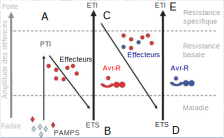
\includegraphics[width=0.8\linewidth]{Evolimunity2}
	\caption[Évolution de l'immunité des plantes d’après le modèle en \og zigzag \fg]{Évolution de l’immunité des 
	 plantes d’après le modèle en \og zigzag \fg, adaptée de \citet{Jones2006}. \\ 
	 A : Les plantes reconnaissent les \glspl{PAMP} (losanges) \textit{via} les
	 récepteurs \glspl{PRR}, ce qui induit la \gls{PTI}. B : Les agents pathogènes sécrètent des facteurs   
	 de virulence (points), qui répriment la \gls{PTI}, permettant la multiplication des agents pathogènes et  
	 conduisant à l’\gls{ETS}. C : Un effecteur  (point rouge) est reconnu spécifiquement par un récepteur (symbole 
	 rouge) codé par un \gls{gene R} de la plante, ce qui active l’\gls{ETI}. D : L’évolution des agents pathogènes  
	 permet l'acquisition de nouveaux effecteurs (en bleu), lui permettant de supprimer l’\gls{ETI} et de déclencher 
	 une nouvelle \gls{ETS}. 
	 E : L’évolution de la plante favorise  de nouveaux \glspl{gene R}, capables de reconnaître les nouveaux 
	 effecteurs, permettant ainsi une nouvelle \gls{ETI}.}
   \label{fig:zigzag}
 \end{figure}
	
      
\subsection{Les résistances qualitatives}
	
	Les résistances qualitatives ou totales sont des résistances monogéniques, reposant sur un \gls{gene R} vis-à-vis d’un agent pathogène. Leur mécanisme d’action  correspond au 
modèle \og gène-pour-gène \fg{}\citep{Flor1971, Moury2010, Thrall2016}.
En 1947, Flor a montré qu'il existe une interaction incompatible entre le lin (\textit{Linum usitatissinum}) et la rouille causée par le champignon\textit{ Melampsora lini}.  Cette relation est basée sur un modèle  gène-pour-gène qui implique qu'un gène d'avirulence (gène \textit{Avr}) chez l’agent pathogène est identifié par un \gls{gene R} chez la plante, entraînant une réaction incompatible, c’est à
dire un blocage de l’agent pathogène par la plante \citep{Dangl2001, Jones2006}; \autoref{tab:GFG}). La reconnaissance très spécifique entre gène \textit{Avr} et \gls{gene R} se produit \textit{via} des récepteurs cytoplasmiques. La résistance qualitative est donc associée à une \gls{ETI}.
Si le \gls{gene R} est inactif ou absent, ou si de manière équivalente le ravageur n'a pas le gène d'\textit{Avr}, l'interaction dite compatible résulte  en une maladie infectieuse. 
	
	
	 \begin{table}[ht]
	    \centering
		  \caption[Modèle d’interaction gène-pour-gène]{Modèle d’interaction gène-pour-gène, 
		           qui stipule qu'un gène 
	     	       avirulent (\textit{Avr}) chez l’agent pathogène est identifié
		           par un gène majeur de résistance  chez la plante.}
		  \label{tab:GFG}
		  
\includegraphics[width=1\linewidth]{GFG2.pdf}  
	 \end{table}
		
	 
	Les \glspl{gene R} sont connus pour de nombreux bioagresseurs  comme des  champignons, oomycètes, virus, bactéries, nématodes et insectes \citep{Dangl2001}. Les  \glspl{gene R}    jouent un rôle important dans le contrôle des maladies 
des céréales comme le blé, le riz et le maïs, mais aussi des cultures maraîchères comme la tomate,
le poivron ou la pomme de terre \citep{Ballvora2002, Hammond-Kosack1997,Schmidt2010, Stuthman2007, Gururani2012, Seid2015,  Pilet2005}.

{\small\medskip \textsc{Remarque --} Le modèle \og matching allele \fg{} est une autre façon de représenter les interactions génétiques entre hôtes et pathogènes. Il suppose que la reconnaissance du pathogène par la plante débouche sur une interaction  compatible, contrairement au modèle gène-pour-gène. L'interaction est généralement fondée sur un seul gène, associé à plusieurs allèles, alors que le modèle gène-pour gène suppose qu'il n'existe que deux allèles (sensible et résistant). Le pathogène peut se développer sur un seul génotype de l'hôte. Dans la version \og inverse matching allele \fg{}, la reconnaissance débouche sur une interaction incompatible, comme le modèle gène-pour-gène, mais toujours pour un seul génotype de l'hôte \citep{Thrall2016}.}


\subsection{Les résistances quantitatives} \label{sec:quantitatives}

	Il existe une autre catégorie  de résistance, les résistances polygéniques  \citep{Cooper1983}. Les traits polygéniques s'expriment sous une forme quantitative  qui peuvent prendre un continuum de valeurs selon les souches
d’agent pathogène, les génotypes de plante et l’environnement \citep{Pariaud2009}.
Les  caractères quantitatifs sont par exemple des caractères mesurables comme le rendement, le taux de succès de l'infection, la période de latence, le taux de croissance. On admet que plusieurs locus ou régions du génome de la plante, portant un ou plusieurs gènes, sont impliqués dans le contrôle de ces caractères et que de nombreux allèles sont responsables de la variabilité. Ces locus sont appelés \gls{QTL}  \citep{Lannou2012}.
On peut noter que lorsque  ces gènes sont associés à la résistance vis-à-vis d’un pathogène, on parle également de \gls{QRL} \citep{Young1996}. Cette résistance polygénique est aussi dite  partielle
ou quantitative,  car elle permet
de ralentir le développement de l’agent pathogène et de baisser l'intensité des symptômes.
Cette résistance est considérée comme  beaucoup plus
fréquente que la résistance qualitative et plus difficile à contourner du fait de son caractère polygénique  \citep{Kearsey1998, Sage-Palloix2007, Parlevliet1989}. 
	
	Bien que   les mécanismes moléculaires sous-jacents à cette résistance polygénique soient encore peu connus, une récente étude a proposé plusieurs mécanismes pouvant contribuer à la mise en place de ce déterminisme polygénique \citep{Poland2009}.
La résistance partielle serait conditionnée par des gènes à effet pléiotrope \footnote{Gène pléiotrope : gène qui détermine plusieurs caractères phénotypiques.}, qui agissent sur la résistance aux pathogènes et sur le
développement des plantes.  
Ceci a été montré pour l'interaction entre \textit{Phytophtora infestans} et pomme de terre, avec la publication de données  sur la colocalisation de \glsplural{QTL} pour la vigueur, la précocité et la
résistance  \citep{Collins1999}.
L’accumulation de composés antimicrobiens au
cours de la \gls{PTI} pourrait ralentir le développement de l’agent pathogène et baisser l’intensité des symptômes. La \gls{PTI} ou la réponse basale serait associée à la résistance  quantitative  \citep{Boller2009}.
Enfin, de nombreux  auteurs considèrent que les facteurs de résistance partielle seraient en réalité  des gènes  majeurs de résistance \og affaiblis \fg{} qui ne permettent pas de stopper complètement le
développement d’un pathogène  \citep{Parlevliet1977, Young1996}. 
Ainsi, \citep{Wang1994} ont  trouvé  des \glsplural{QTL} induisant une résistance partielle dans le pathosystème riz--\textit{Magnaporthe grisea} qui colocalisent avec des \glspl{gene R}. De plus,
lorsqu’un \gls{gene R} a été contourné par une souche de pathogène, ce
gène rendu inefficace permettrait tout de même de réduire le niveau de la maladie. Ce phénomène, appelé  résistance résiduelle  a été rapporté pour plusieurs pathosystèmes \citep{Nass1981, Brodny1986}.

 
\subsection{La  création ou l'amélioration variétale}
 
	L'amélioration variétale classique consiste  à créer de nouvelles variétés à partir de variétés existantes. Elle est apparue avec l'agriculture il y a environ 10\,000 ans.
L'homme cultive alors les plantes  pour son alimentation et pratique une sélection  de manière empirique depuis l'ère néolithique, gardant les graines des plus belles plantes, pour les replanter l'année suivante.
Cela a contribué progressivement à une amélioration de l'espèce cultivée par une sélection  de caractères d'intérêt agronomique  comme la taille des parties consommables (graines, tubercules), les saveurs, la résistance, le rendement. 
L'évolution des techniques de sélection, grâce notamment à la découverte du rôle des organes sexuels chez les végétaux par  Millington-Grew (1676),  des lois  de Gregor Mendel sur la génétique  et l'hérédité \citep{Biffen1905}, des travaux de \citet{Darwin1876}   et de \citep{Shull1908} sur la vigueur des hybrides, ont posé les bases scientifiques de l'amélioration variétale et perpétué cette domestication des plantes. % Au passage, Mendel découvrit ces lois concernant les principes de l'hérédité biologique à partir d'un modèle expérimental sur les petits pois (\textit{Pisum sativum}) en utilisant des procédés d’autofécondations pour produire rapidement un grand nombre de descendants et  %
%À partir des années 1930, l'utilisation de la résistante des plantes   contre
%les bioagresseurs s’est développée de plus en plus \citep{Holmes1938}.  
Les premières variétés hybrides\footnote{Les premières générations d'hybrides (appelé lignées F1) étant hétérozygotes, les semences obtenues à partir de l’autofécondation
de F1 présentent des traits non identiques aux parents. L’utilisation de variétés F1 nécessite donc d’acheter des graines chaque année afin d’hériter des caractères des deux lignées homozygotes pures.} étaient des maïs hybrides, cultivés aux États-Unis à partir des années 1930 \citep{Duvick2001}.
	 
	Aujourd'hui, l'amélioration variétale consiste dans la plupart des  cas  à sélectionner des variétés naturellement résistantes  et de les croiser avec des variétés possédant de bonnes qualités  agronomiques (rendement, vigueur, qualité, valeur nutritive, tolérance aux stress abiotiques) afin de réunir ces caractères dans une seule variété.
Par le choix des meilleures plantes dans la descendance, les sélectionneurs aboutissent après un long travail de sélections successives à la création d'une nouvelle variété, aussi appelée cultivar. Ainsi, les nouveaux cultivars sont tout aussi naturels que les espèces de plantes obtenues par domestication de manière empirique il y a des milliers d'années.  
	
	Lorsqu’un sélectionneur souhaite réaliser l'introgression d'un gène de résistance d'une espèce végétale chez une autre espèce ne possédant pas ce gène, il procède  par croisement  interspécifique
de  deux lignées pures homozygotes  parentales  \citep{Shull1908}, et possédant des caractères d’intérêt qu’il souhaite réunir dans une même lignée. Ce procédé est connu aussi sous le nom d'hybridation. Une fois la lignée \og donneuse \fg{} choisie (ici la lignée résistante), plusieurs rétrocroisements avec la variété cultivée  appelée lignée \og receveuse ou récurrente \fg{} sont  nécessaires pour obtenir une \og  lignée convertie \fg, se rapprochant le plus possible de la variété cultivée mais possédant le gène de résistance.
Cette lignée convertie  sera une lignée pure, stable et reproductible.
L'introgression  du gène \textit{Mi-1} de la tomate vis-à-vis du nématode à galles (genre \textit{Meloidogyne})  en est un exemple typique en culture maraîchère \citep{Milligan1998}. À l'échelle mondiale, c’est le seul gène de résistance actuellement présent dans les variétés de tomate contrôlant plusieurs espèces de nématodes à galles. Ce gène, issu de l’espèce sauvage \textit{Solanum peruvianum}, a été introgressé par croisement interspécifique dans la tomate cultivée \textit{Solanum lycopersicum} et les premières variétés résistantes sont apparues sur le marché à la fin des années 1940 \citep{Smith1944}.
% C’est également de cette manière qu’a été introgressée une résistance chez le blé vis-à-vis du virus \gls{BYDV}  (Sharma et al., 1995).
%Dans le cas du mildiou de la pomme de terre, onze gènes de résistance qualitative identifiés sur l’espèce sauvage \textit{Solanum demissum} ont été  introgressés dans les variétés cultivées \textit{Solanum tuberosum} depuis les années 1950 \citep{Pilet2005, Kuang2005}. 



	L'avancée des connaissances et les progrès technologiques ont permis  la création de nouvelles variétés résistantes, grâce par exemple  au marquage moléculaire et à la transgénèse. %Le marquage  moléculaire  est un marqueur génétique composé de petits fragments d'ADN que l'on appelle amorces ou sondes qui permet de localiser une région particulière du génome de la plante. 
La découverte des marqueurs moléculaires en 1987 et le développement de la PCR (Polymerase Chain Reaction) ont contribué aux premières détections de \glsplural{QTL}. 
La transgénèse correspond, quant à elle, au transfert d'un ou plusieurs gènes provenant d'un cultivar ou d'un autre organisme (bactérie, champignon)  dont l'expression  fait apparaître un caractère  déterminé.  Ces nouvelles variétés sont connues sous le nom d'organismes génétiquement modifiés (OGM). Par exemple,  le maïs \textit{Bt} est une plante transgénique dont la résistance à la pyrale  (un lépidoptère ravageur) est portée par le gène de la bactérie  \textit{Bacillus thuringiensis} (\textit{Bt}) codant la toxine \textit{Cry1Ab}. %  En effet, cette bactérie du sol est mortelle pour la pyrale et  l'innocuité de cette bactérie pour l'homme aurait  été démontrée. %(toutefois des études  continuent à étudier la véracité de cette affirmation).

	%On retrouve comme autre procédé de création variétale, le greffage sur plantes sauvages résistantes. Cette technique semble efficace et particulièrement économique.  Le greffage des légumes est une pratique ancienne. Il a été pratiqué sur certains cucurbitacées  en Chine dès le 1er siècle avant J.C.
%Il s'est vraiment développé à partir de 1920 au Japon avec des porte-greffes courges apportant plus de vigueur aux \textit{Cucurbitacées} telles la pastèque permettant ainsi de diminuer les dégâts. Actuellement, les portes greffes sont  essentiellement utilisés pour les \textit{Solanacées} ($eg.$ tomates et les piments) et les \textit{Cucurbitacées} ($eg.$ melons, concombres, pastèques, courges).

	\begin{figure}[p]
		\centering \includegraphics[width=1\linewidth]{seedvariety.jpg}
		\caption[Perte des variétés ]{Illustration de la perte d’une grande partie 
		         des variétés de fruits et légumes
                 commercialisées entre 1903 à 1983. Source : \citet{NG2011}.}
		\label{loss:varieties}
	\end{figure}

      Au cours du XXème siècle, les sélectionneurs ont créé des nouvelles variétés à partir d'un nombre très limité d'espèce de plantes  d'une culture donnée. 
Cela  a conduit à un appauvrissement important des semences (\autoref{loss:varieties}), de la diversité génétique au sein d'une même espèce  et une plus forte homogénéité dans les paysages agricoles. Par ailleurs, les temps évolutifs entre les agents pathogènes et leurs hôtes sont généralement différent dans les agroécosystèmes. Les agents pathogènes sont généralement à un stade avancé par rapport à leurs hôtes puisqu'ils possèdent un temps de génération plus court et des populations plus importantes, ce qui permet un plus grand nombre de mutations dans une période de temps fixe \citep{Zhan2014}.
Les agroécosystèmes actuels (forte homogénéité des paysages, faible nombres d'espèces de plantes) ont conduit à une évolution uniquement  des agents pathogènes et joue  un rôle majeur dans le contournement des variétés résistantes porteuses de gènes majeurs \citep{Stukenbrock2008}.


\subsection{Contournement et  coût de virulence}
\label{contournement}

	 L'émergence d'agents pathogènes à même de contourner les résistances remet potentiellement en cause l'efficacité de cette méthode de lutte. On parle de contournement de la résistance lorsque tout ou partie de la population d'agents pathogènes s'est adaptée à la résistance et peut dès lors se développer comme s’il s’agissait de plantes sensibles. On parle alors de population \og virulente \fg{} vis-à-vis du gène de résistance concerné \footnote{En biologie évolutive, la virulence est assimilée à la mort de l'hôte due à l'infection. Par souci de clarté dans ce manuscrit, quand on parle de ce type de virulence, on utilise le terme agressivité.} \citep{McDonald2002}. Les \glspl{gene R} sont rares et la plupart des sélectionneurs se concentrent sur l'introgression des principaux \glspl{gene R} dans les variétés végétales \citep{Zhan2015}. Par conséquent, les agriculteurs cultivent finalement la même résistance sur plusieurs années et à grande échelle en monoculture.  Par exemple, en 1969, 85~\% du maïs produit aux États-Unis était de la même variété.
  En 1970, les épidémies  d'helminthosporiose du maïs  (Southern Corn Leaf Blight) et de la \og brûlure jaune des feuilles du maïs \fg{} (Yellow Leaf Blight of Maize) dues respectivement aux champignons \textit{Cochliobolus heterostrophus} (race T) et  \textit{Mycosphaerella zeae-maydis}    ont détruit 17~\% de toutes les cultures de maïs aux États-Unis \citep{Pring1989}.

	 L'introduction de cultivars résistants  provoque un changement des pressions de sélection sur le bioagresseur.  Si un pathogène avirulent perd le gène d'\textit{Avr} à la suite de mutations ou recombinaisons aléatoires, cela peut conduire   à l'émergence et à l'établissement d'un variant pathogène virulent  \citep{McDonald2002, Castagnone-Sereno2002, Garcia-arenal2003a, Parlevliet2002, Moffat2001}. Par la suite, le variant virulent possédant un avantage sélectif par rapport au pathogène avirulent  sur le cultivar résistant, il peut éventuellement s'établir dans la population globale.  En quelques années ou en quelques mois, le bénéfice
fourni par les cultivars résistants peut être annulé en raison de la capacité du pathogène virulent à se propager et à se reproduire \citep{McDonald2002, Parlevliet2002}. Par conséquent, l'agriculture moderne, de par son absence ou manque de diversité génétique chez l'hôte, est  particulièrement exposée aux contournements de résistances et à l’émergence de
nouveaux agents pathogènes \citep{Stukenbrock2008, Anderson2004}. L’identification et l'utilisation accrue de nouveaux cultivars résistants par  les agriculteurs conduit inévitablement à un cycle qui épuise le stock des résistances naturelles des plantes. Ce cycle continu commence par la création d'une nouvelle variété, qui est ensuite déployée jusqu'à une perte quasiment totale de l'efficacité des \glspl{gene R}. Elle est alors remplacée par une nouvelle variété résistante et le cycle recommence... Ce cycle est connu sous le nom de \og boom and bust \fg{} (expansion-récession) \citep{Brown2011, Brown2015, Zhan2015}.

	Pour de nombreux pathosystèmes, l’introduction d’une variété résistante dans un paysage
agricole  conduit souvent à  un  contournement rapide de la résistance par les agents pathogènes. À titre d’exemple, grâce notamment aux travaux de \citet{Moury2010}, le contournement d’une résistance par un virus est un processus bien décrit, qui peut se généraliser à de nombreux pathogènes. Il existe trois étapes
dans le contournement d’une résistance.  La première étape consiste en l’apparition d’un
variant virulent, dans une population avirulente, par une ou plusieurs mutations ou recombinaisons dans un gène d’avirulence (voir Encadrés~\hypertarget{mut2}{\hyperlink{mut1}{La mutation}} et \hypertarget{recomb2}{\hyperlink{recomb1}{La recombinaison}}). 
 Deuxièmement, il faut assurer le maintien de ces mutations
dans la population. Les variants virulents et avirulents sont en compétition et l'issue de cette compétition en faveur des virulents dépend de l’avantage sélectif que ce nouveau caractère leur
procure et de la disponibilité des hôtes compatibles. La fitness de chaque variant, c’est à dire la capacité d’un individu à survivre et à se reproduire, ou encore la capacité d’un individu à transmettre ses gènes à la génération suivante, est un facteur clé pour le maintien et la multiplication des variants virulents. La sélection
des individus les mieux adaptés et la dérive génétique sont deux forces évolutives qui vont
conditionner le maintien d’une population virulente dans un environnement donné \citep{McDonald2002a} (voir Encadrés~\hypertarget{selec2}{\hyperlink{selec1}{La sélection}} et \hypertarget{der2}{\hyperlink{der1}{La dérive}}). La troisième étape se réfère à la capacité de migration du pathogène qui, associée à la sélection et la dérive génétique, permet la fixation du variant dans la population \citep{Brown2002, Charlesworth2009} (voir Encadré~\hypertarget{mig2}{\hyperlink{mig1}{La migration}}).

	Dans la littérature, de nombreux exemples de contournement de résistance ont été signalés.
Par exemple, chez  le phoma du colza (\textit{Leptosphaeria maculans}),  le contournement des résistances \textit{Rlm1}, \textit{Rlm2}, \textit{Rlm4} et \textit{Rlm9} a été démontré après trois ans de culture \citep{Rouxel2005, Rouxel2003}.
Dans le cas du mildiou de la pomme de terre (\textit{P.~infestans}), le contournement des  gènes majeurs de résistance  a été démontré après 5 à 7 ans de culture  \citep{Pilet2005, Kuang2005, Montarry2006}. 
En cultures maraîchères, l’exemple le plus typique est celui du contournement du gène \textit{Mi-1} de la tomate par des nématodes à galles des racines \citep{Castagnone-Sereno2002}. 


\subsubsection*{Coût de virulence}

	La virulence chez la plupart des pathosystèmes est généralement associée à un coût de virulence, appelé également coût de fitness, sur les plantes sensibles et résistantes, qui se traduit souvent par une diminution de la fertilité et/ou de la fécondité \citep{Laine2013, Brown2003} (\autoref{tab:cout}). 
De nombreuses études ont fait état de ce coût de fitness chez des bactéries \citep{Cruz2000, Leach2001}, des oomycètes \citep{Montarry2010}, des virus \citep{Garcia-Arenal2013}
 ou des nématodes \citep{Castagnone-Sereno2002, Castagnone-Sereno2007, Djian-Caporalino2011}. L'existence de coûts de fitness implique que même si les variants virulents sont
sélectionnés sur les cultures résistantes, ils sont  contre-sélectionnés sur les cultures sensibles, où les avirulents  se développent et se reproduisent plus rapidement.

 \begin{table}[ht]
  \centering
   \caption[Interactions entre hôte sensible ou résistant et pathogène avirulent ou virulent, d'après    
          \citet{Leonard1977, Leach2001}]{Interactions entre hôte sensible (susceptible) ou résistant et pathogène  
          avirulent ou virulent, d'après \citet{Leonard1977, Leach2001}. Le succès de l'infection, compris entre 0 (pas 
          d'infection) et 1 (efficacité maximale), peut être réduit par le coût de virulence ($k\in[0,1]$) et 
          l'efficacité de la résistance ($c\in[0,1]$), avec $c=1$ pour une résistance totale/qualitative.}
   \label{tab:cout}
		  \begin{tabular}{c}
		  \includegraphics[width=0.8\linewidth]{Leach.pdf}
		  \end{tabular}
 \end{table}

	L’analyse  des compromis évolutifs pour les modèles gène-pour-gène ont été étudiés par de nombreux auteurs  \citep{Leonard1977, Tellier2007, Brown2015}. Un compromis évolutif peut se définir par  le  choix auquel est contraint un parasite afin de maximiser sa  valeur sélective dans un contexte dans lequel les ressources sont limitées. 
Dans le cas des agroécosystèmes naturels, la coexistence de génotypes de parasites avirulents et virulents en présence d'hôtes sensibles et résistant, résulte d'un compromis évolutif. Ce polymorphisme est dû à des coûts  de virulence qui empêcheraient tout génotype virulent de se diriger vers la fixation \citep{Laine2013}. 


%	\begin{figure}
%		\centering \includegraphics[width=0.7\linewidth]{brown.pdf}
%		\caption{ Illustration de la co-évolution hôte-parasite  impliquant un  simple modèle gène-pour-gène. Source :   \citep{Brown2015} 
%		}
%		\label{co:evolution}
%	\end{figure}

\hypertarget{mut1}{}
\begin{encadre2}{La mutation}
\hyperlink{mut2}{$\curvearrowleft$}
	La mutation correspond à des modifications dans  la séquence
nucléotidique dans le génome d'un individu. Cette force évolutive est la principale source de variation génétique. C’est le mécanisme majeur
d’apparition des virulences, en particulier chez les bactéries et les virus, dont la taille conséquente des populations entraîne  plus grand nombre de mutations \citep{McDonald2002}. Parmi les agents pathogènes des plantes, le taux
de mutation des eucaryotes est compris entre $10^{-9}$ et $10^{-11}$, tandis que chez les bactéries il est
estimé à $10^{-9}$. Les virus montrent des taux de mutation entre $10^{-4}$ et $10^{-8}$ \citep{Drake1998,
Drake1999}. Pour davantage d'exemples, voir \citep{Lynch2010}. 
%Il existe trois types de mutations dites ponctuelles : les mutations par substitution correspondant au changement d’un seul nucléotide,  les mutations par insertion et les mutations par délétion.
\par
Chez les champignons et les bactéries, l’acquisition de
virulences résulte souvent de la délétion ou de l'insertion
d’un fragment d’ADN, qui a pour conséquence l’inactivation du gène d’avirulence
\citep{Kang2001, Gout2007}.
Par exemple, la virulence de certaines souches du champignon \textit{Leptospheria maculans} vis-à-vis du gène de résistance \textit{Rlm1} du colza (\textit{Brassica napus}) est due à une délétion dans le gène d’avirulence \citep{Gout2007}. Chez les virus, l’acquisition de virulence se fait
essentiellement \textit{via} des mutations par substitution nucléotidique et souvent un très
faible nombre de mutations est suffisant pour le contournement de la résistance  \citep{Jenner2000, Moury2004, Janzac2010}. 
Chez les nématodes à galles, l'émergence d'un variant virulent  pourrait être provoquée par des facteurs génétiques et/ou épigénétiques. 
Dans le cas des nématodes à galles (\textit{Meloidogyne}),  des mutations par substitution nucléotidique (ou variations nucléotidiques) ont été trouvées entre
nématodes avirulents et virulents lors d' études expérimentales
\citep{Neveu2003, Semblat2001}. Cependant, très peu de choses sont connues sur les  différents   mécanismes sous-jacents \citep{Castagnone-Sereno1994, Castagnone-sereno2019}.
\end{encadre2}

\hypertarget{recomb1}{}
\begin{encadre2}{La recombinaison}
  \hyperlink{recomb2}{$\curvearrowleft$}
     La recombinaison correspond à un échange d’information génétique entre deux
génomes différents. En fonction du type d'organismes, la
recombinaison se produit de différentes façons :  lors de la reproduction sexuée chez
les eucaryotes, lors de conjugaison bactérienne chez les procaryotes, ou lorsque
plusieurs  virus infectent simultanément une même cellule.
\par
Lorsque  plusieurs allèles de virulence sont nécessaires au contournement d’une résistance (\textit{e.g.} contournement d'un gène pyramidé), la recombinaison accentue les phénomènes de contournement par rapport  à la mutation, car cette dernière nécessite plusieurs événements successifs \citep{McDonald2002}.
\end{encadre2}


\hypertarget{selec1}{}
\begin{encadre2}{La sélection}
  \hyperlink{selec2}{$\curvearrowleft$}
	La sélection fait varier les fréquences alléliques dans les populations et permet de favoriser  les génotypes les mieux  adaptés aux conditions locales. C'est un mécanisme évolutif moteur dans l'évolution des espèces qui permet d'expliquer l'adaptation d'un individu dans un milieu donné \citep{Darwin1859}.
Ce processus évolutif entraîne l’augmentation  ou la diminution  de la fréquence de certains génotypes  en fonction de leur effet sur la reproduction ou la survie des individus (valeur sélective).
% La sélection est la principale force qui détermine les changements de fréquence des allèles mutant \citep{McDonald2002}.
	
	La sélection peut être de trois types : stabilisante, diversifiante ou directionnelle.
La sélection stabilisante permet de favoriser  la fixation des phénotypes moyens par rapport
aux phénotypes extrêmes. On retrouve ce type de sélection au niveau du poids des mammifères à la naissance,
pour lequel deux sélections s’opposent: un poids élevé augmente les chances de
survie  de l'enfant (meilleur accès aux ressources, meilleure défense) mais baisse la
probabilité de survie de la mère, alors qu’un poids faible favorise la survie de la
mère mais diminue la probabilité de survie de l’enfant \citep{Covas2002}.
La sélection diversifiante tend à favoriser la fixation des phénotypes extrêmes par
rapport aux phénotypes moyens. Ce type de sélection a pour conséquence d'éliminer les phénotypes intermédiaires.%L'exemple le plus connu est la taille des becs des pinsons ponceau à ventre
%brun (\textit{Pirenestre ostrinus}). Ces oiseaux 
%peuvent se nourrir de grosses graines ou  de petites en fonction de leur milieu. Seuls les oiseaux possédant un
%gros bec peuvent casser les coquilles dures des grosses graines tandis que les 
%oiseaux à petit bec sont assez adroits pour se saisir des petites. Les oiseaux avec
%un bec intermédiaire possède un désavantage sélectif car ils ne sont pas capables d’ouvrir les
%grosses graines et sont moins habiles  pour se saisir des petites (Smith, 1993). 
La sélection directionnelle tend à favoriser
des  traits phénotypiques (ou génotypiques) d'un extrême par rapport aux autres.
Ce type de sélection est souvent rencontré lorsqu’une population subit  des changements environnementaux abrupts.

	Depuis des  millénaires, les agents pathogènes et les plantes se sont engagés dans une bataille évolutive, les agents pathogènes tentant de surmonter les défenses des plantes et les plantes tentant de résister aux attaques des agents pathogènes \citep{Zhan2015}. 
Dans les écosystèmes naturels, ces processus co-évolutifs
ont permis de retarder et/ou diminuer les épidémies grâce à une hétérogénéité spatiale et/ou temporelle de l’environnement  \citep{Zhan2015, Burdon2014}. 
L’introduction à grande échelle d’un cultivar portant un gène de résistance à un agent pathogène   induit une pression de sélection directionnelle sur l'agent pathogène ciblé. 
La monoculture peut être ainsi considérée comme une pression de sélection directionnelle en faveur des individus virulents capables d’infecter les plantes porteuses du gène de résistance.% En effet,
L'utilisation de pesticides chimiques peut conduire également à une sélection directionnelle \citep{Pimentel1985}.
\end{encadre2}

\hypertarget{der1}{}
\begin{encadre2}{La dérive génétique}
  \hyperlink{der2}{$\curvearrowleft$}
La dérive génétique correspond à des fluctuations aléatoires de la fréquence des génotypes au sein d’une même population \citep{Henry1999}. 
La dérive génétique a comme conséquence la perte d’allèles et donc la  réduction de la variabilité génétique. La dérive génétique influence les dynamiques évolutives indépendamment des génotypes présents dans la population, car elle repose sur un processus aléatoire (contrairement à la \hyperlink{selec1}{sélection}).
\par
Il est important d’introduire le concept de taille efficace d’une population pour illustrer les conséquences de la dérive génétique. La taille efficace correspond au nombre d’individus au sein d’une population  transmettant de manière \og efficace \fg{} leurs gènes à leurs descendants.  Ainsi, la taille efficace d’une population peut être définie comme la taille d'une population \og idéale\fg{} présentant les mêmes fluctuations de fréquences d'allèles que la population étudiée  \citep{Gutierrez2012}.
La taille efficace est généralement plus petite que la taille réelle de la population \citep{Charlesworth2009}. 
 Plus la taille efficace est petite, plus l’effet de la dérive est élevé et donc plus la perte de  variabilité génétique est grande \citep{McDonald2002}. En particulier, pour des populations  soumises à la dérive génétique (notamment chez les virus), une petite taille efficace peut mener à la perte de mutations associées à la virulence et ainsi éviter ou réduire les risques  de contournement d'une résistance, augmentant ainsi sa durabilité \citep{Rousseau2019}.
\end{encadre2}

\hypertarget{mig1}{}
	\begin{encadre2}{La migration}
\hyperlink{mig2}{$\curvearrowleft$}
      La migration  est un processus par lequel des allèles (gènes) ou des individus (génotypes) particuliers sont échangés entre des populations géographiquement séparées \citep{McDonald2002}.
Dans un système de populations interconnectées, les nouvelles
mutations conférant un avantage adaptatif peuvent ainsi se propager entre les populations \citep{Burdon1999}.
\par
Ce phénomène peut entraîner l’arrivée de pathogènes virulents dans une culture où ils sont initialement absents, à cause de la présence de variants à proximité de la culture  (\textit{e.g.} plantes sauvages). L'homme peut aussi être à l'origine de la migration d'agents pathogènes, à cause de pratiques culturales par exemple  \citep{Brown2002, Burdon1993}. Ainsi, la dispersion d'agents pathogènes peut être possible au-delà des capacités naturelles de dispersion de ces derniers.  
\end{encadre2}


\section{Durabilité des résistances} \label{durabilite}
    
\subsection{Définitions}
	
	\citet{Johnson1984} a défini qu’une résistance était durable lorsqu’elle restait efficace suite à son déploiement sur une longue durée et à grande échelle, dans un environnement favorable au développement
du pathogène. %Ainsi, on peut quantifier la durabilité d’une résistance après un
%déploiement de la résistance sur un horizon temporel long et dans la plupart du temps une fois
%que la résistance ai été contournée  \citep{Johnson1981}. 
%La durabilité d’une résistance est donc fortement corrélée avec le contournement de la résistance.
%La durabilité va donc principalement dépendre du temps nécessaire pour l'acquisition d'une ou plusieurs  mutations chez l'agent pathogène et de la capacité des agents pathogènes virulents à s'établir dans la population (mode de reproduction, mode de dispersion, taille des populations) (Barrett et al,
%2008 ; Brown, 2015 ; Macdonald2002,  Stuthman et al, 2007 ; van den Bosch et al, 2007.
%Gilligan, 2003 ; Zhan et al, 2015).
La durabilité d’une résistance diffère  en fonction des systèmes hôtes-pathogènes. Plus une résistance est difficilement contournable, plus elle est durable.
La résistance qualitative aux maladies des plantes est connue pour avoir une faible durabilité vis-à-vis des pathogènes fongiques, bactériens et viraux \citep{Garcia-Arenal2003, Brown2015, Parlevliet2002}. Néanmoins, il existe des gènes de résistance qualitative durable comme le gène \textit{Tm2} chez la tomate et le gène \textit{N} chez le tabac contre le tobacco mosaic virus pour lesquels on n'a pas observé de contournement   \citep{Parlevliet2002}.
Par ailleurs, il a été démontré qu'une résistance quantitative serait plus durable qu'une résistance qualitative \citep{Mundt2014, Palloix2009}. Par exemple, la résistance à la rouille des feuilles de l'orge (\textit{Puccinia hordei}) observée chez les cultivars d'orge Minerva et Vada est une résistance  polygénique qui est aussi efficace aujourd'hui que lors de sa première utilisation en \textit{1955} \citep{Parlevliet2002}. 
Pour les nématodes (du genre \textit{Meloidogyne}), le
gène de résistance \textit{Mi-1} commercialisé depuis 60 ans, procure une durabilité assez stable \citep{Williamson2006}, bien que des contournements aient été observés ces dernières décennies à l'échelle mondiale  \citep{Castagnone-Sereno2002, Verdejo-Lucas2009,Seid2015}. 

	La définition de la durabilité par \citet{Johnson1984} est qualitative \footnote{La définition de la durabilité par \citet{Johnson1984} ne permet pas de mesurer la durabilité d'une résistance de manière quantitative et ainsi de comparer les durabilités.}. 
Il existe également des métriques quantitatives de durabilité, en lien avec des critères comme la fréquence d'agents pathogènes virulents ou encore le rendement. On retrouve dans la littérature des approches expérimentales pour mesurer la durabilité.
\citet{Barbary2014}, par exemple, ont étudié la durabilité des \glspl{gene R} \textit{Me1}  et \textit{Me3}  aux nématodes \textit{Meloidogyne incognita} en inoculant des nématodes avrirulents à très forte concentration puis en calculant le pourcentage de plantes présentant plus de 5 galles. Ce seuil permet de déterminer si la résistance a été contournée ou non. 
Cependant, dans un modèle \og gène-pour-gène  \fg, la durabilité d'une résistance dépend du temps nécessaire pour l'acquisition d'une ou plusieurs  mutations chez l'agent pathogène et de la capacité des agents pathogènes virulents à s'établir dans la population hôte sur des échelles spatiales plus ou moins larges \citep{Barrett2008, Brown2015, McDonald2002,  Stuthman2007, vandenBosch2003, Zhan2015}. Cette capacité dépend en particulier du niveau d’agrégation spatiale et/ou temporelle des variétés hôtes, ainsi que de la structure et la dynamique démo-génétique de la population de pathogènes (qui dépend du mode  et du taux de reproduction, de la dispersion, de la taille des populations, des coûts de fitness, \textit{etc.}). La prise en compte des facteurs épidémiologiques, démographiques, génétiques  et de leurs interactions  est donc importante pour quantifier la durabilité d'une résistance. Ceci est difficilement réalisable par des approches expérimentales à cause du temps et du coût de la mise en place d'expériences de terrain à grande échelle.

	Les approches de modélisation mathématique permettent d'évaluer et/ou de comparer l'efficacité et la durabilité des résistances, sur des échelles de temps longues et des échelles spatiales allant de la plante au paysage agricole. \citet{vandenBosch2003} ont proposé, à partir d’un modèle mathématique, trois mesures quantitatives de la durabilité : (i) le nombre d’hôtes non infectés  jusqu’à ce que  la résistance soit contournée,
c’est à dire que la fréquence de virulents ait dépassé un certain seuil ; (ii) le temps écoulé entre
l’introduction du cultivar résistant et le moment où la fréquence de pathogènes virulents, présents initialement, atteint un seuil prédéfini, par exemple 90~\% ; (iii) le délai d’invasion, c’est-à-dire la durée nécessaire au  pathogène virulent pour envahir les cultures de plantes résistantes, sachant qu’il est absent
de la parcelle avant l’introduction de la résistance. 
La plupart des modèles de la littérature utilisent la définition (ii) \citep{vandenBosch2003, Fabre2015, Lof2017}.

%La fréquence seuil de virulents au-delà de laquelle la résistance est considérée comme contournée est clairement arbitraire et dépend de facteurs socio-économiques \citep{Bourguet2016}.

	Dans le \autoref{article}, nous avons défini la durabilité comme le nombre de saisons au bout duquel une stratégie de déploiement composée uniquement de plantes résistantes engendre une perte de rendement relative par rapport au temps initial (\textit{i.e.} la première année de culture) supérieure à un seuil prédéfini, par exemple 1~\%. Cette mesure de durabilité est fondée sur le rendement des cultures et non la fréquence des virulents, comme dans les trois mesures proposées. 	
		
% Cette thèse a comme but la recherche  de stratégies optimales de déploiement des résistances en utilisant des principes éco-évolutifs afin d'améliorer leur efficacité et leur durabilité. Ces principes permettent de retarder l'évolution des pathogènes et d'augmenter significativement les rendements des cultures, sans l'utilisation des pesticides chimiques. L'identification de ces stratégies pourra permettre de mieux gérer le déploiement des résistances dans les agroécosystèmes et  une meilleur protection des résistances naturelles des plantes.
	 Nous allons exposer dans la suite  comment augmenter la durabilité des résistances
et le rendement des cultures à long terme grâce à des stratégies basées sur des principes
éco-évolutifs qui permettent de retarder l’émergence et/ou l’établissement des populations
virulentes  \citep{Zhan2015, Zhan2014, Brown2015, Bourguet2016}.
	 
    
\subsection[Comment améliorer la durabilité et l'efficacité des résistances variétales ?]{Comment améliorer la durabilité et l'efficacité des résistances des plantes dans les agroécosystèmes ?}
\label{durabilite_sub}

	Favoriser l'hétérogénéité spatiale et/ou temporelle des pressions de sélection dans les agroécosystèmes est la méthode la plus prometteuse afin de gérer durablement le déploiement de la résistance des plantes \citep{Zhan2015, Brown2015, Bourguet2016}. Ces stratégies sont similaires  à celles utilisées pour retarder l'évolution de la résistance aux médicaments et aux pesticides \citep{Bourguet2016, Consortium2013}.
On peut citer principalement quatre stratégies  :
(1) la combinaison de
plusieurs gènes de résistance dans la même plante (pyramidage) ; (2) l'utilisation de 
différents cultivars au sein d'un même champ (mélanges) ou  (3) entre les champs (mosaïques) ;
(4) l'alternance dans le temps de cultivars différents (rotation).
De nombreuses études expérimentales et de modélisation ont démontré l'effet bénéfique de ces stratégies pour augmenter le  rendement des cultures  et la durabilité des résistances \citep{Fabre2012,  Djian-Caporalino2014, Mundt2014, Fabre2015, Bourguet2016}. En outre, de rares études expérimentales  \citep{Djian-Caporalino2014} et différents travaux de modélisation \citep{Bourguet2016, Lof2017, Rimbaud2018} ont comparé la durabilité de ces stratégies. Sur la base des résultats  menées sur la gestion des résistances aux pesticides et aux médicaments \citep{Consortium2013}, \citet{Bourguet2016} hiérarchisent les stratégies en termes de durabilité des résistances aux maladies comme suit : 
pyramidage $>$ mélanges de variétés et mosaïques  $=$ rotation $>$ usage d'une résistance qualitative en monoculture. Toutefois, de nombreuses études ont démontré qu'il n'existe pas de stratégie universellement meilleure que les autres en termes de durabilité \citep{Rimbaud2018, Fabre2012, Djidjou-Demasse2017}. Par exemple, \citet{Sapoukhina2009}, par une approche de modélisation du déploiement spatial des gènes de résistance, a constaté que le pyramidage était tout aussi efficace qu'un mélange aléatoire de cultivars résistants monogéniques. Nous allons voir dans la suite et de manière plus détaillé, les différentes stratégies pour le contrôle des agents pathogènes et pour augmenter la durabilité des résistances des plantes. 
 
\subsubsection{Le pyramidage} \label{sec:durabilite_pyramidage}

	La stratégie la plus courante  consiste à pyramider plusieurs gènes de résistance majeurs en un seul cultivar, dans l'espoir que l'agent pathogène ne puisse pas facilement acquérir la séquence de mutations lui permettant de contourner les différents  gènes de résistance \citep{McDonald2002}.  
Dans sa revue, \citet{Mundt2018} retrace plus en détails le succès du pyramidage.
Le dogme standard a été que, si les gènes de résistance n'ont pas encore été déployés individuellement, la probabilité qu'un agent pathogène asexué acquière le facteur de  virulence contre tous les gènes de résistance pyramidés est très faible  \citep{Schafer1985}.
L'efficacité du pyramidage de \glspl{gene R} repose sur plusieurs hypothèses clés, sans lesquelles elle pourrait être compromise  : (1)
les mutations pour l'acquisition de la virulence sont indépendantes, (2) les virulences ne sont pas préexistantes dans la population de l'agent pathogène, (3) la résistance conférée par chaque gène pyramidé n'a pas encore été contournée, (4) les gènes de résistance  ont  des modes d'action non redondants \citep{Bourguet2016}.
%Il a été démontré que les gènes d'avirulence agissent également comme effecteurs de la virulence et qu'il existe une redondance considérable entre les effecteurs \citep{Jones2006, Cunnac2011}. 
 Par ailleurs, \citet{Leach2001} soutiennent  qu'il existe une relation de cause à effet entre le coût de fitness associé à la virulence  et la durabilité des \glspl{gene R} correspondants.
Ils ont donc émis l'hypothèse que, le pyramidage de gènes ayant un coût de fitness élevé, il devrait être durable.
 Il est attendu que la recombinaison dans le génome d'un agent pathogène soit un mécanisme susceptible de désavantager cette stratégie \citep{Burdon2014, Mundt2014, Brown2015}, car l'agent pathogène pourrait combiner par la suite des mutations présentes dans différents variants du pathogène pour contourner la résistance.

	
	\citet{Rimbaud2018} ont utilisé un modèle mathématique stochastique afin d'évaluer la durabilité du pyramidage de deux \glspl{gene R} pour le contrôle d'une maladie fongique.
Ils ont montré que le pyramidage  est très durable et efficace, car contourner cette résistance totale nécessiterait l'acquisition simultanée de virulences aux deux \glspl{gene R} à forts coûts de fitness.
%Cette stratégie permet de diminuer les risques de contournement et d'augmenter la durabilité des résistances par rapport au déploiement d'un seul gène de résistance \citep{Vu2014, Mundt2018, Pink2002}. 
\citet{Rimbaud2018a}, dans une nouvelle étude, ont comparé les quatre  principales stratégies de déploiement de la résistance des céréales à la rouille (\textit{Puccinia}). Ils ont montré que le pyramidage de gènes était moins  susceptible d'être contourné, mais que les conséquences pourraient être  désastreuses si cela se produisait. En effet, à long terme la forte pression de sélection directionnelle induit une adaptation de l'agent pathogène sur l’ensemble des résistances qualitatives pyramidées; cela conduit à l'émergence d'un variant double-virulent  et  à une perte de l'efficacité des résistances qualitatives (notamment en absence de coût de fitness \citep{Lof2017}). Par exemple, deux gènes de résistance qualitative  pyramidés de  la tomate vis-à-vis du champignon \textit{Cladosporium fulvum} ont été  simultanément contournés suite à l’apparition de pathogènes double-virulents, rendant inefficace toutes les résistances qualitatives \citep{Lindhout2002}.
	
	Des études ont démontré que la combinaison des résistances quantitatives avec une résistance qualitative fournit une meilleure protection des gènes majeurs de résistance \citep{Palloix2009, Brun2010, Delourme2014}. Ces études testent l'efficacité et/ou la durabilité de cultivars résistants impliquant l'introgression d'un \gls{gene R} dans des fonds génétiques \og résistants \fg{} (résistance quantitative). Ainsi,  \citet{Palloix2009} ont  démontré pour  l'interaction piment (\textit{Capsicum annuum}) –  \gls{PVY} que la durabilité du gène de résistance  \textit{pvr2}$^3$  dépendait du fond génétique de la plante dans lequel il était introgressé. \citet{Quenouille2014}, par une étude expérimentale  ont ensuite démontré que l'amélioration de la durabilité correspondait à des \glspl{QTL} de résistance présents dans le fond génétique. Cet effet pourrait résulter d'une réduction de la probabilité de fixation des mutations  bénéfiques pour le virus. Autre exemple, le pyramidage d’un gène de
résistance qualitative \textit{Rlm6}  avec des résistances partielles a montré une durabilité plus intéressante par rapport à une résistance qualitative seule chez le colza \textit{Brassica
napus}  vis-à-vis du champignon \textit{Leptosphaeria maculans} \citep{Brun2010}.
Pour les nématodes à galles, la résistance partielle du piment vis-à-vis des nématodes à galles permet également d'améliorer 
la durabilité ainsi que l'efficacité des \glspl{gene R}  \citep{Barbary2014}.
Cette  plus forte durabilité s'explique  vraisemblablement  par le fait que la résistance quantitative est polygénique, alors que la résistance qualitative dépend d'un seul gène de résistance majeur \citep{Mundt2014, Parlevliet1989}. La résistance polygénique permet de relâcher la  sélection qui s'opère sur les agents pathogènes virulents, contrairement à une résistance qualitative où la sélection est unidirectionnelle \citep{Quenouille2014, Bourguet2016}.

	Dans une autre étude de modélisation, \citet{Rousseau2019} ont étudié l’effet de stratégies de mélanges variétaux dans le but d’augmenter la durabilité des résistances aux virus. Le paysage agricole qu’ils ont étudié comprenait  deux variétés de plantes en mélange, une sensible et une résistante, et deux variants pathogènes, un avirulent et un virulent. 
Dans cette étude, ils ont testé  si la combinaison d'une résistance quantitative réduisant le goulot d'étranglement de la population virale (diminution du $Ne$) avec une résistance qualitative peut augmenter la durabilité de cette dernière. 
Ils ont comparé  les rendements d'un mélange de cultivars sensibles et résistants combinant une résistance qualitative avec une résistance quantitative (pyramidage) et d'un autre comprenant des cultivars sensibles et résistants portant une résistance qualitative (résistance monogénique).
Ils ont montré que les rendements d'un mélange avec la variété pyramidée étaient plus notables  qu'un mélange avec la variété résistante portant un \gls{gene R} pour des coûts de fitness intermédiaires. La stratégie optimale impliquant la résistance pyramidée pourrait fournir jusqu'à 95 \%  de rendement supplémentaire par rapport à un mélange impliquant la résistance qualitative seule.% En effet,
%pour les coûts de fitness élevés, la résistance était durable si bien que le rendement de la stratégie optimale
%ne pouvait être que marginalement augmenté. À l’inverse, pour les faibles coûts de fitness la résistance était
%inefficace et n’apportait aucun bénéfice dans la stratégie optimale. Pour des coûts de fitness intermédiaire, la résistance quantitative contrôlant la taille des goulots d'étranglement peut protéger une résistance qualitative en diminuant la probabilité de succès de la transmission de l'infection des plantes sensibles infectées aux plantes résistantes saines (voir encadré  \hyperlink{der1}{\hypertarget{der2}{La dérive}}) }.

	En conclusion, l'efficacité de cette stratégie seule repose sur le fait que l'acquisition de plusieurs virulences  est très difficile et qu'elle est très probablement associée à de forts coûts de fitness \citep{Brown2015, Leach2001, Fabre2009, Janzac2009}. 


\subsubsection{Les mélanges et mosaïques}
\label{subsubsec:mel}

	L'hétérogénéité des hôtes peut être assurée par  mélanges de différents cultivars  au sein d'une même parcelle  ou entre les parcelles (mosaïques de cultivars) \citep{Keesing2006, Mccallum2015}. Ces stratégies  permettent  de limiter les risques de contournement des résistances des plantes en jouant sur les pressions sélectives. L'idée standard qui contribue au  succès de cette stratégie est qu'elle perturbe la sélection directionnelle, en favorisant différents allèles ou génotypes virulents à différents endroits, retardant par conséquent la montée en fréquence de l'allèle ou du génotype virulent \citep{McDonald2002}. 
Les mélanges et les mosaïques de cultivars contribuent ainsi à améliorer le contrôle épidémiologique et la durabilité des résistances \citep{Burdon2016, Burdon2014}.
	
	Différents modèles théoriques et expériences ont pu démontrer l’effet bénéfique des mélanges de cultivars hôtes en termes de contrôle épidémiologique \citep{Zhu2000,  Mundt2002, Wolfe1985, Kiyosawa1982, Garrett1999}.
Dans sa revue,  \citep{Mundt2002} détaille notamment plusieurs facteurs influençant l'effet des mélanges pour le contrôle des maladies dans un paysage agricole.
Premièrement, on s'attend à ce que l'efficacité des mélanges diminue avec la proportion d’autoinfections\footnote{L'autoinfection  signifie que le parasite est né dans l'hôte qu'il infecte, alors que l'alloinfection signifie que le parasite est arrivé d'ailleurs et qu'il a donc dû se déplacer vers son hôte. La première infection de tout individu hôte sain doit être une alloinfection.}, qui est influencée à la fois par les caractéristiques de l'agent pathogène et de l'hôte.
Deuxièmement, des modèles mathématiques ont montré que l'efficacité des mélanges décroissait
avec la capacité de dispersion de l’agent pathogène \citep{Fitt1986}. 
Troisièmement, des expériences en conditions contrôlées et des études numériques ont montré que l'efficacité des mélanges était moindre pour les parasites générant de grandes lésions, à cause d'une saturation des  plantes infectées \citep{Lannou1994}. 

 %Au delà  de ces facteurs assez généraux, nous verrons dans la suite que  lorsque l'on considère  une stratégie de mélange ou de mosaïque entre cultivars sensibles et résistants, d'autres  facteurs comme le ratio de plantes résistantes, l'hétérogénéité spatiale des hôtes  jouent un rôle très important dans le succès de la stratégie. 
	
	Dans les agroécosystèmes,  le but des mélanges variétaux peut être  de protéger les cultivars sensibles, en les combinant avec des cultivars résistants. En effet, les variants avirulents ne peuvent pas se développer sur  les plantes résistantes et l'existence de coûts de fitness implique que les virulents sont contre-sélectionnés sur les cultures sensibles. Le mélange des deux cultivars permet de combiner ces deux effets et ainsi de contrôler les variants avirulents et virulents.
Cette relation entre la diversité des hôtes et la transmission de la maladie s'explique principalement par un effet de dilution \citep{Mundt2002}.   L'augmentation de la diversité génétique des cultures devrait réduire le taux de transmission des agents pathogènes et diminuer l'intensité des épidémies \citep{Mundt2002}.
Plusieurs approches visant à améliorer la durabilité des \glspl{gene R} sur la base de combinaisons appropriées de cultivars de plantes résistantes et sensibles ont été proposées \citep{vandenBosch2003, LoIacono2012, Fabre2012,  Fabre2015, Lof2017}.
Différents modèles théoriques et expériences   ont pu démontrer l’effet bénéfique de l’hétérogénéité phénotypique avec le mélange de plusieurs cultivars hôtes pour un contrôle épidémiologique  \citep{Mundt2002, Wolfe1985, Kiyosawa1982, Zhu2000}.
	
	\citet{Fabre2012}, à travers une étude numérique,  ont quantifié l'effet de différents  facteurs qui influencent les pertes de rendement d'une stratégie de mélange entre un cultivar sensible et un cultivar résistant à un virus. Ils ont montré que lorsque les  infections se faisaient principalement entre parcelles, la proportion optimale de plantes résistantes dans la stratégie  de mélange était de 50~\%. Par contre, dans les paysages où les infections se faisaient principalement depuis le réservoir, les stratégies de résistance pures étaient également pertinentes. En outre, les auteurs ont montré que l'efficacité des mélanges pour contrôler une maladie virale et augmenter la durabilité des résistances  dépend également de l’intensité
des épidémies et des caractéristiques du \gls{gene R}.  \citet{vandenBosch2003}, ont démontré 
pour le contrôle d'un agent pathogène foliaire, que la durabilité des \glspl{gene R} est généralement préservée en utilisant un faible ratio de  résistance.  \citet{Djidjou-Demasse2017} ont conduit une étude théorique à partir d'un modèle démo-génétique, de l'échelle d'une plante jusqu'à l'échelle du paysage afin de comparer une stratégie de pyramidage  avec une stratégie de mosaïque pour le contrôle d'une maladie virale. Ils ont montré que la stratégie de mosaïque était optimale  quand  les infections d'un champ à l'autre prédominaient, les intensités épidémiques  étaient élevées et les coûts de fitness associés à la virulence étaient faibles.
	
	L'efficacité de cette stratégie de lutte contre les maladies foliaires a été démontrée en premier lieu  sans tenir compte de la distribution spatiale des hôtes et des pathogènes \citep{Browning1969}.
En se basant sur  des études expérimentales et des simulations, \citet{Mundt1985} ont montré comment l'arrangement spatial des génotypes hôtes affecte l'efficacité  des mélanges variétaux.
Ils ont montré que l'efficacité du mélange diminue lorsque le degré d'agrégation des génotypes végétaux augmente dans un mélange de plantes sensibles et résistantes  \citep{Mundt1986, Mundt1986b}. Par exemple, les mélanges de culture de riz au japon contrôlent  mieux la pyriculariose causée par le champignon \textit{Magnaporthe grisea} lorsque le mélange variétal est au sein des collines  plutôt qu'entre collines.

	 À travers un modèle à l'échelle du paysage, \citet{Papaix2014} ont étudié l’effet du niveau d'agrégation spatiale des hôtes et du type de résistance sur le contrôle d’une maladie foliaire due
à un agent pathogène transmis par voie aérienne. 
Différents paysages, composés de deux variétés, une
sensible et une résistante, ont été analysés. Les paysages avec un faible niveau d'agrégation étaient plus efficaces  pour contrôler l'épidémie lors du déploiement
d’une variété doté d'une résistance qualitative. En revanche, dans le cas  d'une variété dotée d'une résistance
quantitative,  des paysages plus agrégés pouvaient se révéler plus efficaces, selon la proportion de plantes résistantes et leur niveau de résistance.

En ce qui concerne les nématodes à galles, les mélanges variétaux de lignée résistantes  semblent peu efficaces pour protéger les cultures sensibles aux nématodes sur le long terme  \citep{Djian-Caporalino2014}, notamment  à cause de la faible dispersion intrinsèque de ce type de parasite. 

	En conclusion,  cela fait maintenant plus de 60 ans que l'appel en faveur de l'utilisation de cultivars résistants dans un déploiement assurant de la diversité génétique a été lancé \citep{Jensen1952}. Les mélanges ont connu des succès majeurs pour lutter contre les maladies, mais leur effet dépend de certaines conditions épidémiologiques (proportion d'autoinfections, capacité de dispersion).  Les questions d'échelles spatiales, qui sont déterminées par les interactions hôtes-pathogènes, peuvent  être cruciales pour évaluer l'utilité potentielle des mélanges en termes de  contrôle épidémiologique et de durabilité des résistances.



\subsubsection{Les rotations}

	La rotation des cultures consiste à alterner différentes espèces ou cultivars dans le temps. C'est l'une des plus anciennes stratégies de gestion appliquées par les agriculteurs, pour améliorer  la fertilisation des sols et gérer les populations nuisibles \citep{Bullock1992,Bruns2012}. Elle diminue les coûts de production et améliore l'environnement, en réduisant les émissions de gaz à effet de serre et l'utilisation des pesticides \citep{Kleijn2019,Bargues-Ribera2020}.
L'utilisation des rotations entre plantes hôtes et non hôtes (de différentes espèces) est souvent réalisée en grande culture pour des raisons agronomiques, \textit{e.g.} blé-colza-soja. 
La séquence de culture la plus simple pour la gestion des dégâts causés par un pathogène  est celle dans laquelle la culture hôte est cultivée pendant un an  seulement, après quoi les cultures non hôtes sont plantées pendant une ou plusieurs années consécutives, puis la culture hôte est à nouveau plantée pendant une seule année. 
Il existe également des rotations de cultures entre cultivars résistants uniquement ou entre cultivars sensibles et résistants. Dans ce cas, les rotations des cultures permettent de modifier la montée en fréquence de pathogènes virulents afin
de freiner leur développement et de les maintenir sous un seuil de nuisibilité acceptable. 
	
	L'utilisation de cette stratégie  perturbe la sélection directionnelle en favorisant différents allèles ou génotypes mutants à différents moments, réduisant ainsi la vitesse à laquelle ils augmentent en fréquence \citep{McDonald2002}.
%À travers des modèles mathématiques ou des expérimentations sur terrains, il est possible d'étudier comment les populations d'agents pathogènes sont affectées par l'alternance de pressions sélectives  dans le temps.  La dynamique des populations d'agents pathogènes à tendance à diminuer sur le long terme lorsque les différents cultivars hôtes  varient dans le temps, puisque les taux de  reproduction (et/ou d'infection) sont différents pour chaque cultivar hôte.
Par exemple, si les pathogènes virulents sont sélectionnés en cas d'usage de plantes résistantes, ils sont contre-sélectionnés en cas d'usage de plantes sensibles au profit de pathogènes avirulents qui ont généralement une meilleure fitness. L’intensité de cette contre-sélection dépend des coût de fitness dans l’adaptation du variant virulent aux différents hôtes \citep{Zhan2015, Brown2015, Brown2011}. 
%La mise en place de rotation de culture entre cultivar résistant et sensible permet donc de diminuer la montée en fréquence  des pathogènes  virulents et d'augmenter la durabilité des résistances.

	L’évolution continue du pathogène  a souvent été mise en relation avec la notion de cycles d'expansion-récession (boom-and-bust cycles) \citep{Brown2015, McDonald2002, Zhan2015}. La  rotation des cultures dans le temps permet de rompre ce cycle, en diminuant la pression de sélection sur les populations virulentes,  de telle sorte  qu'elles ne ne se développent pas  (\autoref{rotation}).  Le succès de la rotation repose  également sur le fait que l'agent pathogène ciblé  se disperse peu d'une année à l'autre.  Par ailleurs, une stratégie de rotation efficace doit s'assurer que les populations virulentes sont en très faibles proportions au moment de l'introduction du cultivar résistant, afin de profiter pleinement de l'efficacité de la résistance.
%De plus, l'absence apparente de virulence croisée est un facteur très important dans la réussite de cette stratégie Fournet2013.


\begin{figure}
	\centering 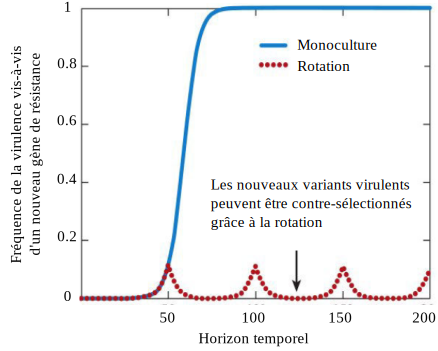
\includegraphics[width=0.8\linewidth]{rotation.pdf}
		\caption[Évolution  d’un agent pathogène vis-à-vis d'une plante porteuse d’un
		nouveau gène de résistance en monoculture  ou avec une rotation
		des cultures]{Évolution  d’un agent pathogène vis-à-vis d'une plante porteuse d’un
		nouveau gène de résistance en monoculture (courbe bleue), ou avec une rotation
		des cultures (courbe en pointillés rouges).  Adapté de \citep{Zhan2015}.
		}
		\label{rotation}
\end{figure}


%Dans les domaines de la santé publique et de l’agronomie, REX Consortium (2013) ont mis en avant l’intérêt des combinaisons entre mélange de molécules et leurs rotations dans le temps pour la gestion de la résistance conférée par les insecticides ou antibiotiques aux ravageurs et aux agents pathogènes, après avoir analysé un ensemble de 29 études théoriques sur le sujet. Ces études comparaient cette stratégie double (mélange et rotation) à des stratégies plus simples, consistant (i) en un mélange de molécules constant dans le temps, ou (ii) en une alternance temporelle entre différentes molécules utilisées une par une séparément, soit de manière cyclique, soit en changeant de molécule lorsque celle en cours d’utilisation était contournée. REX Consortium (2013) ont conclu que les stratégies combinant mélange et rotations étaient au moins aussi performantes, voire plus performantes que les autres stratégies pour retarder le contournement d’une résistance dans plus de 80~\% des comparaisons.
 Selon \citet{Zhan2015}, il existe encore trop peu d’études théoriques pour la conception et l’évaluation de stratégies  de gestion durable des maladies, notamment pour celles basées sur la rotation de \glspl{gene R} \citep{Fabre2015, Papaix2015, Lof2017, Rimbaud2018}. 
À partir d'une approche de modélisation, \citet{Fabre2015}  ont montré que les rotations et les mosaïques combinées  étaient plus bénéfiques que les mosaïques seules en termes de rendement lorsque des infections se déroulent majoritairement au sein d'une même parcelle, c'est-à-dire quand la capacité de dispersion de l'agent pathogène est faible, et pour des variants  où le contournement de la résistance vis à vis d'un virus se faisait après une seule mutation. Les auteurs ont aussi montré une augmentation de la durabilité des résistances grâce au maintien de  la fréquence des variants virulents sous un certain seuil.

	\citet{Rimbaud2018} ont trouvé que la rotation des cultivars peut être la plus efficace à long terme par rapport aux trois autres stratégies de déploiement (pyramidage, mélanges, mosaïques), une fois que tous les \glspl{gene R} ont été contournés. Cependant, ils ont montré que ce résultat dépend au moins en partie de la capacité de dispersion et de survie des agents pathogènes.  Un pathogène avec une grande capacité de dispersion aura tendance à diminuer l'efficacité de cette stratégie car le pathogène pourra se propager pour infecter d'autres champs. L'efficacité de la rotation   seule pourrait être limitée dans les régions où la culture est pratiquée sur de grandes superficies, en particulier pour les maladies propagées par voie aérienne.

%\tr{Je dois aussi présenter Zhu 2000 \citep{Zhu2000})}  
	 Certaines ont montré l’efficacité des rotations basées sur l'alternance de cultivars sensibles et résistants  pour lutter contre des pathogènes qui se dispersent peu, notamment contre les nématodes à galles \citep{McSorley2011, Miller2006, Tzortzakakis2000}. Une autre étude, menée sur la tomate en Espagne durant trois ans, a montré que cette alternance pouvait augmenter les rendements et la durabilité de la résistance des plantes  \citep{Talavera2009}. Quelques  études expérimentales ont évalué l'effet bénéfique des rotations pour différents types de pathosystèmes \citep{Zhu2000, Talavera2009, Djian-Caporalino2014, Burdon2014}. 

	 Au sein de notre laboratoire,  \citet{Djian-Caporalino2014} ont évalué et comparé expérimentalement sur trois ans  la  durabilité et l'efficacité de trois stratégies de déploiement des \glspl{gene R} chez le piment pour lutter contre les  nématodes à  galles \textit{Meloidogyne},  parasites telluriques peu mobiles :
le mélange de cultivars, les rotations  et le pyramidage de deux \glspl{gene R} dans un même cultivar. 
En s'assurant de l'absence  de virulence croisée, ils ont montré que l'alternance du \gls{gene R}  \textit{Me3} avec un autre \gls{gene R} à  mode d'action différent  \textit{Me1} chez le piment semble efficace pour réduire les populations de nématodes. Cette  efficacité pourrait reposer sur la spécificité de la virulence des gènes \textit{Me1 } et \textit{Me3},  démontrée en conditions contrôlées \citep{Djian-Caporalino2011} :  si une population peut contourner un \gls{gene R} (par exemple \textit{Me3} à résistance précoce), en revanche elle ne peut contourner un autre \gls{gene R} (par exemple le gène \textit{Me1} à résistance tardive).

%Les rotations  permettent d'éviter que les populations  ne soient soumises à des pressions de sélection constantes et n’évoluent rapidement vers la virulence (comme dans l'exemple de la \autoref{rotation}).

	
	Les nématodes à galles, évoqués à plusieurs reprises jusqu'ici, ont été choisi comme cas d'étude  dans cette thèse. Ils sont présentés  de façon plus détaillée dans la section suivante.

%\printbibliography[heading=subbibliography,segment=\therefsegment]

\section{Cas d'étude : les nématodes à galles } \label{nematode}

\subsection{Qu'est ce qu’un nématode ?}
	
\begin{figure}[h]
  \centering \includegraphics[width=1\linewidth]{schema_nem}
	  \caption[Schéma général d’un nématode]{Schéma général d’un nématode. \href{https://www.wormatlas.org/}{https://  
	  www.wormatlas.org/}}
	  \label{nematodes}
\end{figure}
	
	Les nématodes sont des vers ronds, non segmentés, filiformes et translucides (\autoref{nematodes}), qui appartiennent à l'embranchement des Nematoda, dont plus de 25000 espèces réparties  dans 20 ordres et 200 familles ont été identifiées jusqu'à présent \citep{Abad2008}.  Toutefois, on estime à plus d’un million le nombre d’espèces existantes de nématodes \citep{Hugot2001}. Ce sont des métazoaires. %tripoblastiques pseudocoelomates.
Dans le règne animal, ils représentent une grande partie de la biodiversité animale, juste après les insectes  qui constituent 80~\% de cette biodiversité. 
Ils s'acclimatent à pratiquement tous types d'environnements et sont donc distribués partout dans le monde. Les nématodes  ont réussi à s'adapter à de larges gammes d'écosystèmes et milieux : eau, sol, animaux, champignons, insectes et  plantes \citep{Bongers1998}. Certains d'entre eux participent de manière fondamentale à l'activité biologique dans divers écosystèmes. Ils jouent un rôle important dans la décomposition de déchets organiques, y compris dans la biodégradation de composés toxiques. La présence de nématodes dans les sols peut  même être un indicateur de la qualité du sol \citep{Yeates1987}.


\subsection{Les nématodes phytoparasites}
	
	Plus de  4500 espèces de nématodes phytoparasites ont été découvertes à ce jour \citep{Decraemer2006}.
Ils sont répartis dans deux ordres : celui des \textit{Dorylaimida} qui comprend les nématodes vecteurs de virus \citep{Maheswari1997} et celui des \textit{Tylenchida} qui est
l’ordre le plus important par le nombre d’espèces,  qui causent d'importants dégâts aux cultures \citep{DeGuiran1983}.
Ils mesurent tous  moins d'un millimètre de long et sont invisibles à l’œil nu.
La principale caractéristique des nématodes phytoparasites est un stylet perforant se situant dans la  partie antérieure du tube digestif. C’est une aiguille creuse
connectée à un système glandulaire hypertrophié, qui agit comme une véritable pompe en injectant des sécrétions nécessaires au parasitisme et en absorbant les nutriments
de la plante \citep{Abad2010}.  Les nématodes phytoparasites sont responsables de 11~\% de la perte de
production  des cultures vivrières \citep{Agrios2005}. Globalement, ils sont responsables de 10~\% à 20~\% de pertes de rendement sur toutes cultures confondues\citep{Raaijmakers2009}.
Les pertes annuelles mondiales seraient
estimées à plus de 100 milliards d’euros \citep{Sasser1987, Chitwood2003}. D'autres études menées 20 ans plus tard ont confirmé ces chiffres \citep{McCarter2009, Chitwood2003, Agrios2005}.
	
	De par leur comportement, il existe deux types de parasitisme : (1) les parasites aériens qui s'attaquent aux bulbes, tiges, feuilles, fleurs des plantes et (2) les parasites des racines qui peuvent être ectoparasites \footnote{se dit d'un parasite qui vit  à la surface des tissus végétaux, animaux ou humains} ou endoparasites, migrateurs  ou sédentaires.  

	Parmi les nématodes phytoparasites, les nématodes parasites des racines sont probablement la principale cause de pertes de récoltes, mais également ce sont  les plus représentés à l'échelle du globe \citep{Bird2003}.  Les nématodes phytoparasites des racines réalisent tout leur cycle de vie dans le sol et ne s’attaquent qu’aux
racines ce qui peut conduire à un dysfonctionnement du système vasculaire de la plante, voire à la mort de la plante selon le stade et les taux d’infestation. 
Les symptômes de l'infection par des nématodes des racines sont : 
	\begin{itemize}[label=--]
	\item des apparitions de galles ou de lésions racinaires qui favorisent d'autres pathogènes telluriques, fongiques 
	      ou bactériens ;
	\item une distorsion de la structure racinaire ou une augmentation du diamètre des racines ;
	\item une croissance racinaire réduite (perte racinaire) ou une  nécrose des racines pouvant entraîner la mort de 
	     la plante.
	\end{itemize}
Par exemple, les nématodes  endoparasites migrateurs pénètrent complètement et se déplacent dans les tissus parasités  des racines entraînant des lésions (genre : \textit{Ditylenchus, Pratylenchus, Rotylenchus}). Les nématodes endoparasites sédentaires pénètrent dans les tissus et se sédentarisent pour établir un site nourricier pour leur développement, entraînant la formation à terme de galles ou de kystes.

La majorité des pertes de récoltes sont causées par les nématodes endoparasites sédentaires, qui comprennent les nématodes à kystes (genres \textit{Heterodera, Globodera})  \citep{Perry2018} et les  nématodes à galles (genre \textit{Meloidogyne}) \citep{Perry2009}, ainsi que les endoparasites migrateurs, qui comprennent par exemple les nématodes à lésions des racines (genre \textit{Pratylenchus}) \citep{Mass1998}. 
 
\subsection{Les nématodes à galles du genre \textit{Meloidogyne}}
	
	Les nématodes à galles du genre \textit{Meloidogyne} sont des endoparasites obligatoires des racines. Du fait de leur taille microscopique et de leur présence au sein même des racines, ils sont longtemps passés inaperçus.  Ils créent des galles au niveau des racines, entraînant une déformation importante du système vasculaire  de la plante, mais aussi  un dépérissement des parties aériennes et parfois la mort de plante.

	Ils sont particulièrement nuisibles économiquement aux cultures agricoles du monde entier en raison de leur large gamme d'hôtes, comprenant plus de 5500 espèces de plantes \citep{Blok2008}, et de leur large répartition géographique \citep{Jones2013}.  En cas d’infestation forte, les galles peuvent envahir tout le système racinaire, ce qui provoque une diminution des rendements de la plante  et  peut conduire dans certains cas à la perte totale d’une récolte. En effet, les racines attaquées par les nématodes ne sont plus capables d’extraire correctement des nutriments du sol et donc de se développer (\autoref{degat}).  Les dommages  de certaines espèces de \textit{Meloidogyne} ont été répertoriés par \citet{Greco2010} et \citet{Wesemael2011}.  Par exemple, des pertes de rendement de 62 à 100~\% ont été signalées en culture de tomates sensibles  \citep{Seid2015, Gine2017}, 30 à 60~\% en cultures d'aubergine, 50~\% pour le melon,  37~\% à 50~\% pour la  pastèque \citep{Sikora2005} et 88~\% pour les concombres \citep{Gine2017}. 
En Europe, ils sont responsables de dégâts atteignant 10\% de la production céréalière et ils  entraînent des diminutions de récoltes de 20 à 30\% dans les vergers d'agrumes méditerranéens \citep{Feldmesser1971}.  Dans le sud-est de la France,  plus de 40\% des exploitations maraîchères sont touchées \citep{Djian-Caporalino2010, Djian-Caporalino2012}.
Le changement climatique est susceptible d'influencer nettement  la distribution de ces parasites et par conséquent d'accentuer les pertes de rendement des  cultures \citep{Bebber2014}. 

	\begin{figure}
	    \centering
		  
\includegraphics[width=0.9\linewidth]{degat}
		  \caption[Dégâts provoqués par \textit{ Meloidogyne incognita}]{Dégâts provoqués par \textit{ Meloidogyne 
		   incognita} sur : \textbf{A} des racines de tomates ;
		   \textbf{B}  une culture en serre d’aubergines ; \textbf{C} 
		   des racines de haricots.}
		  \label{degat}
	\end{figure}

	Plus de de 90 espèces ont été décrites \citep{Jones2013, Blok2008}, dont 23 en Europe \citep{Wesemael2011}, mais seulement quatre d'entre elles sont considérées comme particulièrement nuisibles : \textit{M.~incognita, M.~arenaria, M.~javanica} et  \textit{M.~hapla}. En France, on retrouve principalement les trois premières de ces quatre espèces.  Ces trois espèces sont à reproduction parthénogénétique mitotique   (c'est à dire à reproduction clonale) \citep{Triantaphyllou1985}. Elles sont responsables de
la majorité des pertes de rendement des cultures maraîchères causées par les
nématodes \citep{Sikora2005}. Elles sont également largement répandues dans les régions tropicales, où elles s’attaquent aux cultures de
bananier, de café, de coton de canne à sucre ou encore d’ananas \citep{Sikora2018}. Elles  prospèrent dans les sols des contrées à climat chaud et hivers courts.

	L'espèce \textit{Meloidogyne incognita} est   l'une des espèces les plus largement répandues à travers le monde et celle qui cause le plus de dégâts. \textit{M.~incognita} se distingue par son caractère extrêmement polyphage. Elle attaque plus de 200 espèces végétales, dont les tomates, aubergines, poivrons, pommes de terre, melons, concombres, laitues, chicorées, haricots, carottes, \textit{etc.} 
	Dans ce contexte, certains auteurs indiquent que \textit{M. incognita} serait l'un des parasites de plantes parmi les plus préoccupants au monde \citep{Bebber2014}. 	
	

\subsection{Le cycle de vie du nématode \textit{M. incognita}}
\label{sec:cycle}
 
 
Le cycle biologique  du nématode se déroule en  deux phases décrites ci-dessous.

\paragraph{La phase exophyte}

	Les œufs sont produits dans une matrice gélatineuse à la surface des racines.  Chaque œuf présent dans le sol libère directement une larve de deuxième stade (J2),  la  mue J1--J2 ayant lieu dans
l’enveloppe de l’œuf. Les larves ont une apparence vermiforme et sont la plupart du temps translucides ou de couleur claire. Elles sont mobiles dans le sol et, attirées par les
exsudats racinaires, elles pénètrent à l’intérieur de leur hôte. On parle aussi de stade infestant ou de larves infestantes \autoref{larve}.

	\begin{figure}
	  \centering
		  \includegraphics[width=0.7\linewidth]{J2}
		  \caption[Larve de deuxième stade de \textit{M. incognita}]{\textbf{A}  Schéma de la partie antérieure d’une   
		          J2 de \textit{Meloidogyne} d’après \citet{Vanholme2004}.
		           Stades de développement  de \textit{M. incognita}. \textbf{B} Juvéniles du deuxième stade  
		           \textit{M.incognita} observées à la loupe binoculaire (source : photos Inrae Sophia Antipolis).}
		 \label{larve}
	\end{figure}

\paragraph{La phase endophyte}
Cette pénétration a lieu préférentiellement au niveau de l’apex (extrémité) des racines en croissance et constitue le début d'une phase où le nématode va se sédentariser dans les racines de la plante entre le 3 ième et le 4 ième jours. En effet,  les larves J2 migrent dans la racine pour remonter vers le cylindre central de la plante et initier un site nourricier potentiel. Les J2 instaurent un site nourricier composé en général de 5 à 6 cellules géantes plurinucléées \footnote{se dit d'une cellule qui renferme plusieurs noyaux}  pour les assister dans leur parasitisme, en sécrétant des salives  et d’autres métabolites. 
Une fois établi, le parasite n'a plus besoin de se déplacer pour accomplir son cycle \citep{Abad2010}. Grâce à son stylet buccal, il ponctionne les cellules géantes et aspire leur contenu pour se nourrir.
%Cette larve J2 subit alors deux mues successives qui la mènent au troisième (J3), puis au quatrième stade larvaire (J4). 
		
	 Après 3 mues, les larves J3 puis J4 deviennent des femelles matures qui  produisent alors une masse d’œufs gélatineuse à l'extérieur de la racine.
Chaque femelle peut produire environs un millier d’œufs \citep{Castagnone-Sereno2013}, qui vont démarrer un nouveau cycle.
%Plus précisément dans le cadre de cette thèse,   nous nous sommes basé sur des publications dans lequel le potentiel reproducteur d'une femelle \textit{Meloidogyne incognita} pouvait être compris entre 250 et 300 œufs \citep{Castagnone-sereno2007, Djian-Caporalino2011}. 
Le cycle complet  (\autoref{cycle}) s’effectue en moyenne entre  20 à 24 jours à 25$^{\circ}$. Le cycle peut durer jusqu'à 40 jours selon la température.
Chez les espèces \textit{M. incognita} qui sont à reproduction  parthénogénétique, les mâles peuvent être très rares et ne participent pas à la reproduction \citep{Triantaphyllou1979}. La présence des mâles est plus élevée lorsque  les  J2 sont confrontées à des conditions défavorables de développement (\textit{e.g.} mauvais état des racines nourricières de la plante hôte). 
Contrairement aux J2 et femelles, les mâles ne se nourrissent pas et quittent la racine. Par ailleurs, le taux d’éclosion de l’espèce \textit{M. incognita} peut être total dans les conditions environnementales optimales. Mais il est en généralement  compris entre 60~\% et 80~\% dans les conditions expérimentales \citep{DeGuiran1979}. %Par exemple, nous avons constaté
%que dans les conditions expérimentales de l'Ehwaeti et al \citep{Ehwaeti1998} que le taux d’éclosion était de 73~\% \citep{Ehwaeti1998}.
%Nous avons donc déduit que la femelle pond 17 oeufs viables en moyenne au cours de sa durée de vie, qui est comprise entre 8 à 10 jours (Ekanayake and Vito, 1986).
La survie naturelle  dans le sol en absence de nourriture à 25 $^\circ$ C est de 25 jours, les J2  mobilisant l’ensemble de leurs réserves énergétiques avant de mourir \citep{Tsai2008}.
Les population de \textit{M. incognita} peuvent néanmoins se maintenir en infectant
les adventices hôtes ou des débris de racines dans le sol.
Enfin, les œufs  peuvent survivre des semaines ou des  mois  $via$ des stratégies telles que le retard de l'embryogenèse, la diapause ou encore des états de quiescence qui prolongent leur viabilité \citep{Perry2009}. 


\begin{figure}
	\centering \includegraphics[width=0.8\linewidth]{cycle_de_vie3}
		\caption[Cycle de vie du nématode à galles \textit{Meloidogyne} \textit{incognita} dans une racine (Photos  
		Inrae Sophia Antipolis).]{Cycle de vie du nématode à galles \textit{Meloidogyne} incognita dans une racine.  La 
		larve juvénile mobile de deuxième stade  (J2)
      	migre après 24h  en moyenne vers l'extrémité d'une racine (A)  avant de remonter le long du cylindre central au  
      	bout de trois jours (B) et atteindre l’emplacement du futur site nourricier (C-C').
	    Les stades juvéniles J3  et J4  fixés sont visibles en coupe racinaire avec les cellules géantes (*)  au bout 
	    du 10 ième et 14 ième jours respectivement (D-E).% Ces troisième et quatrième stades larvaires  ne se nourrissent pas et n’ont pas de stylet.
	    La larve (J4) muent alors une dernière fois pour produire un adulte, soit  mâle (F) ou femelle (G). La femelle 
	    mature est visible au  bout du 20 ième jour et produit une masses d'oeufs  à l'extérieur de la racine au bout 
	    du 24 ième jour (H). Adapté de \citet{Abad2008}.}
	   \label{cycle}
\end{figure}

\newpage
 
\subsection{Moyens de lutte} \label{lutte}
	
\subsubsection{La lutte chimique}

	La lutte contre les nématodes à galles a longtemps été restreinte  à l'utilisation de produits chimiques.
Tout d'abord, on retrouve  des gaz toxiques (fumigants), tels que des produits
organo-halogénés (bromure de méthyle, 1,3-dichloropropène) ou de la famille des
thiocyanates (métham-sodium, dazomet) \citep{Wesemael2011}. Ensuite, il existe  des nématicides systémiques (non-fumigants) tels que
des carbamates (aldicarbe, oxamyl, carbofuran) ou des organophosphorés (éthoprophos,
phénamiphos, fosthiazate, terbufos) \citep{Cavelier1987}. Ces produits qui se diffusent par la sève, tuent le nématode par ingestion. Toutefois, ils sont interdits sur toute culture comestible.

	L'utilisation de ces produits chimiques n'était efficace que sur de faibles profondeurs et ils n'étaient donc pas efficaces dans les couches profondes du sol.
Depuis 2006, beaucoup de ces produits chimiques ont été retirés du marché à cause de leur impact environnemental et sanitaire \citep{Abad2010}. C'est par exemple le cas du  bromure de méthyle qui a été interdit par l'UE \citep*{MBTOC2006, ECDirective2009}. 

\subsubsection{Prophylaxie et lutte physique}
		
	 La prophylaxie (hygiène des parcelles) consiste d'une part à  enlever un maximum de déchets et de racines pour que les parasites évitent de trouver de quoi se nourrir et d'autre part à détruire les adventices aux abords des parcelles, les mauvais herbes constituant un réservoir pour la multiplication des nématodes. D'autre moyens, physiques, sont utilisés pour nettoyer les sols  comme la solarisation  (\autoref{solarisation}). C'est un procédé qui consiste à inonder le sol  puis à le   recouvrir d'une bâche plastique transparente    afin de permettre de faire monter sa température jusqu’à 50$^{\circ}$C selon le principe de l'effet de serre  \citep{Porter1983}.
	
	\begin{figure}
		\centering \includegraphics[width=0.8\linewidth]{solarisation.jpg}
		\caption{Solarisation en plein champ et sous abri (photo GRAB).}
		\label{solarisation}
	\end{figure}
	
	Si cette technique a démontré son efficacité pour le contrôle des agents pathogènes fongiques,  utilisée seule elle est  peu efficace  contre les nématodes à galles et doit être renouvelée tous les 2-3 ans \citep{Anastasiadis2008}. Si la température n’est pas assez élevée en profondeur, dans certains cas (petites surfaces, sols sableux, équipement disponible), on peut utiliser la désinfection à la vapeur. Celle-ci permet d’injecter de la vapeur sous une bâche étanche recouvrant le sol pendant 1h30 à 3h. La profondeur traitée est de dix à vingt centimètres lorsque le sol est finement préparé. Cette méthode est néanmoins coûteuse et polluante (fluel).
%	\begin{figure}
	%	\centering \includegraphics[width=0.8\linewidth]{desinfection-vapeur.png}
		%\caption{ Désinfection à la vapeur (photos Inra Sophia Antipolis).
		%}
		%\label{solarisation}
	%\end{figure}
	
	
\subsubsection{La lutte culturale} \label{lutte:culturale}
		
	La lutte culturale est une méthode de lutte  qui vise à limiter le développement des parasites/pathogènes  en jouant sur leur environnement naturel et en perturbant leur cycle biologique. Elle peut inclure, de manière non exhaustive,  la gestion de l'irrigation, les rotations culturales, les plantes pièges.
La gestion de l'irrigation permet d'éviter la dissémination des nématodes par ravinement et donc une meilleur protection des cultures au champs. Le labour  profond estival peut
permettre de faire remonter les  nématodes des couches profondes du sol qui vont
sécher en surface. Néanmoins, un labour systématique a pour conséquence une diminution de la quantité de matière organique du sol.
Les rotations culturales bien réalisées jouent un rôle important dans la lutte contre les nématodes. 
Pour freiner le développement des nématodes on peut inclure dans les rotations des espèces végétales
mauvais hôtes vis-à-vis des nématodes à galles ($e.g.$ \textit{Liliaceae}, \textit{Brassicaceae}),  biofulmigantes ($e.g.$ sorgho,  \textit{Brassicaceae}) ou des  plantes pièges ($e.g.$ radis fourragers) en interculture \citep{Djian-Caporalino2019}. 
Les  plantes biofumigantes  produisent des phytoanticipines qui agissent comme
des inhibiteurs de développement ou des toxines. La culture de plante pièges consiste à planter un bon hôte pendant une courte période, suffisante pour assurer une forte pénétration des nématodes et un développement du nématode.  Ensuite, les racines doivent être enlevées ou détruites afin de tuer les nématodes avant la reproduction (dans le cas de plantes pièges résistantes la culture n'est pas détruite en générale ce qui n'est pas le cas de cultures sensibles). Par exemple,  certaines variétés de piments et melons 
  vont  attirer les  nématodes  et permettent la pénétration des larves de \textit{Meloidogyne} mais pas leur développement en femelles fécondes \citep{Berge1974, Djian-Caporalino2008}. L'utilisation de ces plantes de service fait l'objet de récents projets \citep{Djian-Caporalino2019}.
	
	


%4.2. Lutte biologique

%Certains antagonistes du sol tels que les bactéries et les champignons prédateurs peuvent être utilisés comme agents de lutte biologique contre les nématodes (Ritter, 1985 ; Robinson, 1999). Ce type de pratique présente cependant la difficulté de maintenir un auxiliaire dans un sol qui ne lui convient pas toujours. Cette méthode de lutte est donc très loin d’être appliquée à grande échelle.

	
\subsubsection{La lutte génétique}


	\begin{figure}[H]
		\centering \includegraphics[scale=0.4]{RvsS.pdf}
		\caption[Comparaison de
l’interaction des nématodes
à galles entre une plante
sensible et résistante]{ Comparaison de
l’interaction des nématodes
à galles avec A) une tomate
sensible B)  et une tomate
résistante   \textit{Mi-1}, C) un piment résistant \textit{Me1}  (photos
INRAE Sophia Antipolis).  Adapté de \citet{Djian-Caporalino2015}.}
 		\label{RvsS}
	\end{figure}




	La résistance qualitative ou totale est une méthode  efficace, respectueuse de l'environnement et économiquement viable dans la lutte contre les nématodes  du genre \textit{ Meloidogyne} \citep{Roberts1982, Roberts1990, Roberts1993, Williamson2009, Davies2015, Barbary2015}. Les mécanismes d'interaction du modèle gène pour gène, qui se traduit par un \gls{HR} en cas d'interaction incompatible (\autoref{RvsS}),  ont été décrits pour les nématodes à galles \citep{Kombrink2001, Pegard2005, Williamson2006}. Le nématode, une fois dans les racines, produit des substances chimiques  reconnues spécifiquement par un \gls{gene R} de la plante.


	Cependant, l'utilisation de la résistance aux nématodes  à galles se heurte à plusieurs problèmes. Tout d'abord, à
	ce jour, seulement une trentaine de  gènes de résistance vis-à-vis des différentes espèces de \textit{Meloidogyne}  ont été identifiés (\autoref{tab:resistance}). En particulier, il existe peu de résistances naturelles conférant une résistance totale aux nématodes à galles   :  la
carotte (gène \textit{Mj-1}), les prunus (gènes \textit{Ma}), la tomate
(gènes \textit{Mi}), la pomme de terre (gènes \textit{Rmc1},
\textit{MfaXII}),  le coton (gènes \textit{MIC-3,
rkn-1, Mi-1}), les piments/poivrons (gène \textit{N} et
gènes\textit{ Me} ) \citep{Djian-Caporalino2008}.
%La plupart  des cultivars  ont été obtenus par introgression  d'un nombre limité de cultivars naturellement résistants ou de portes-greffes \og  courges \fg{}  apportant plus de vigueur aux Cucurbitacées.

\begin{table}
	\caption[Résumé des gènes de résistance aux nématodes à galles]{Un résumé des gènes de résistance aux nématodes à  
	 galles (\textit{Meloidogyne}),  d'après \citet{Williamson2009}.}
	\centering
	\begin{tabular}{c}
	\includegraphics[width=1\linewidth]{tab_res.pdf}\\
	\end{tabular}
	\label{tab:resistance}
\end{table}

	
	Ensuite, les résistances peuvent être contournées par des populations  de \textit{Meloidogyne} qui évoluent plus ou moins rapidement \citep{Castagnone-Sereno2002, Verdejo-Lucas2009,Jarquin-Barberena1991}.  
Pour mettre en évidence, ce succès parasitaire surprenant malgré l'absence de recombinaisons sexuels et génétiques de nombreuses études expérimentales  ont travaillé sur ces questions de contournement.
Premièrement, la virulence des nématodes à galles  vis-à-vis d'un gène de résistance pourrait être due  à des  variations nucléotidiques entre
nématodes avirulents et virulents 
\citep{Neveu2003, Semblat2001}.Deuxièmement,
des chercheurs se sont intéressés  aux variations des copies de gènes dans les régions du génome d'un variant virulent comparativement à celui d'un variant avirulent pour tenter d'expliquer l'apparition du variant virulent \citep{Castagnone-sereno2019}. Leur étude a montré qu'il existe des régions du génome uniquement représentés chez les lignées avirulentes et absent sur les lignées virulentes. Ainsi, la perte de gènes chez le variant virulent  pourrait être un élément clef dans l'acquisition de la virulence. Ces résultats et/ou également  d'autre facteurs génétiques telles des  inversions, des translocations ou des éléments transposables  dans le génome de \textit{Meloidogyne}  pourraient expliquer l'apparition du variant virulent. Troisièmement, des chercheurs de notre laboratoire soupçonnent que des modifications épigénétiques  pourraient provoquer des modifications au niveau du génome qui sont connus aujourd'hui pour être des facteurs déterminants dans l'acquisition de nouveaux traits.
	
	 Cependant, on connaît très peu de choses sur les modifications génétiques et épigénétiques impliquées dans l'acquisition de la virulence chez \textit{Meloidogyne} 
De ce fait,  le taux de mutation des nématodes \textit{M.} \textit{incognita} reste encore inconnu. À titre d'exemple, le taux de mutation du nématode \textit{C. elegans}  est  de l'ordre de  10$^{-6}$ \citep{Denver2004}. 
En revanche, le taux d'apparition d'individus virulents dans une population avirulente (ou  la fréquence d'apparition de phénotype virulent dans une population avirulente)  serait plus proche de  10$^{-3}$ \citep{Castagnone-Sereno1994}.
	 
	 Le problème du contournement  est particulièrement préoccupant pour le gène de la tomate \textit{Mi-1} qui est à l'heure actuelle le seul  présent dans toutes les variétés de tomates commercialisées dans le monde. Pour cette raison, un changement de variété au cours du temps ne modifierait pas la pression de sélection appliquée sur les populations de parasites, puisque \textit{in fine} le gène de résistance resterait le même. 
L'étude de la sélection vers  la virulence a été menée dans  l'interaction entre \textit{M. incognita} et la tomate résistance \textit{Mi-1}  \citep{Castagnone-Sereno2002, Castagnone-Sereno2007}. Le contournement de ce gène a donc été mis en évidence, ce qui remet potentiellement en question la durabilité de cette méthode \citep{Castagnone-Sereno2002}.
 
 
	 
	L’analyse des traits d’histoire de vie des nématodes, lorsque les nématodes  sont inoculés à des génotypes sensibles ou résistants, montre qu’il existe un coût  associé à l'acquisition de la virulence. En effet, la virulence chez les nématodes \textit{M. incognita} est  associée à un coût de fitness sur les plantes sensibles, représenté par une diminution de la reproduction et de la fertilité \citep{Castagnone-Sereno2007, Djian-Caporalino2011} (\autoref{cost}). Ainsi, si les nématodes virulents sont sélectionnés en cas d'usage de plantes résistantes, ils sont aussi contre-sélectionnés en cas d'usage de plantes sensibles au profit de nématodes avirulents.
Dans l'étude de  \citet{Castagnone-Sereno2007}, les coûts de virulence peuvent être calculés selon la formule suivante :
\begin{equation}
 Ch(\%) = 1-RP_v/RP_{av} 
 \end{equation}
où $RP_v$ est le potentiel reproducteur  (nombre d’œufs / nombre de larves inoculées) de la lignée virulente et $ RP_{av} $  est le potentiel reproducteur  de la lignée avirulente  sur tomate sensible  \citep{Castagnone-Sereno2007}. 
À partir de cette formule, nous avons estimé le coût de virulence sur tomates sensibles
à 31~\%  pour la reproduction  et  à 9~\% pour la fertilité.

\begin{figure}
	\centering 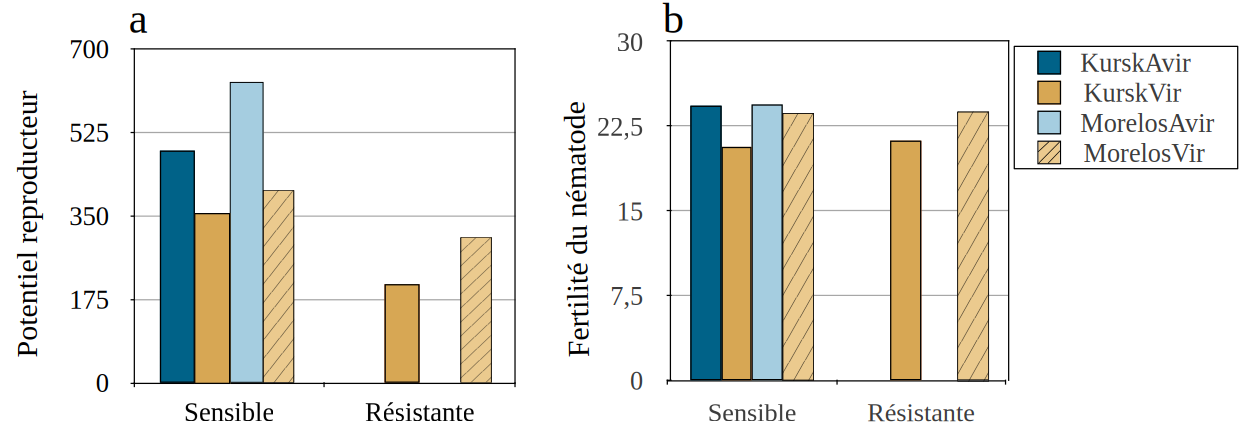
\includegraphics[width=1\linewidth]{cost2.pdf}
	\caption[a) Potentiel reproducteur et b) fertilité des nématodes \textit{Meloidogyne} \textit{incognita}. ]{ a)  
	 Potentiel reproducteur (nombre d'oeufs viables / larves inoculées) de M. \textit{incognita} sur tomates sensibles  
	 (\textit{cv.} Saint Pierre) et \textit{Mi} résistantes (\textit{cv.} Piersol). b) Nombre de femelles de M. 
	 \textit{ incognita} ayant produit une ponte par larve inoculée  sur plantes sensibles et résistantes. KurskAvir et 
	 MorelosAvir représentent les lignés avirulentes ; KurskVir et MorelosVir représentent les lignés virulentes.   
	 Adapté de \citet{Castagnone-Sereno2007}.}
	\label{cost}
\end{figure}



	
	En conclusion, des solutions alternatives à la lutte chimique existent (solarisation, biofumigation, désinfection vapeur, plante piège), mais prises individuellement elles, restent insuffisantes en termes d’efficacité  pour une augmentation significative des rendements. La résistance des plantes est une stratégie efficace et peu coûteuse pour le contrôle des nématodes à galles. La réponse immune des plantes est principalement représentée par les \glspl{gene R} dans le cas des nématodes à galles  dont l’utilisation est de plus en plus compromise à cause du nombre limité de
variétés résistantes et de la faible durabilité de certains \glspl{gene R}.
Il paraît plus que nécessaire de  mettre l'accent sur des études qui suggèrent une gestion plus durable du nombre limité et irremplaçable de résistances encore disponibles vis-à-vis des nématodes à galles.

\textit{
Dans cette thèse, nous avons identifié des rotations de cultures sensibles et résistantes pour augmenter les rendements, mais également pour préserver les rares et précieux \glspl{gene R} disponibles.}

%Dans l'infection par les nématodes, il existe différents types de réponses  des résistances chez les plantes. Notamment, chez le piment il existe deux gènes
%majeurs de résistance aux nématodes à mécanismes d’action différents (\autoref{RvsS}) : l’un (\textit{Me3}) agit de manière
%précoce et l’autre (\textit{Me1}) de manière plus tardive. Dans la suite, nous aborderons la spécificité de ces modes d'action dans le pathosystème piment-\textit{Meloidogyne} et leur lien avec la durabilité des \glspl{gene R}. 
\newpage
\subsection{Les gènes majeurs de résistance \textit{Me(s)} du piment aux nématodes à galles}

\label{sec:gene-R-piment}

\begin{encadre2}{Le piment : origine}
\label{pim}Le terme vernaculaire \og piment \fg{} regroupe l’ensemble des plantes du genre \textit{Capsicum} appartenant à la même famille des \textit{Solanaceae} que la tomate, la pomme de terre, l’aubergine et le tabac. Le genre regroupe environ vingt-cinq espèces différentes avec des différences au niveau de la forme, de la couleur du goût, de la puissance du piquant et de la taille.

\parbox{7cm}{%
\begin{figure}[H]
\hspace{3.5cm}
\includegraphics[width=0.4\linewidth]{piment.png}	

 \begin{minipage}{0.96\linewidth}
 \caption[Collection de piments de l’INRAE d’Avignon, France (Photos Inrae sophia Antipolis)]{Diversité 
      de formes et couleurs de fruit chez \textit{C.}  \textit{annuum} (échantillon de la collection de 
  piment de l’INRAE d’Avignon, France) }
 \label{piments}
 \end{minipage}	
\end{figure}
}
Parmi elles, seules cinq ont été domestiquées :
\textit{Capsicum annuum, C. frutescens, C. chinense, C. pubescens} et \textit{C. baccatum.}
Le piment a été domestiqué pour la première fois en Amérique.
Des traces archéologiques ont montré que  les piments font partie de l'alimentation des peuples d'Amérique depuis au moins 8000 ans \citep{Aguilar-Melendez2009}. L'introduction de l'espèce \textit{C. annuum} en Europe pour la première fois date du XVe siècle, lorsque Christophe Colomb le ramena de son
premier voyage. Cette espèce est maintenant la plus cultivée au monde 
Il s’agit d’une culture maraîchère qui produit des petits fruits forts et « brûlants »
ainsi que des fruits plus gros et doux couramment appelés \og poivrons \fg . Cette espèce est originaire
du Mexique, du Sud de la Bolivie et du Brésil, on la retrouve maintenant dans les régions tropicales à travers le monde et dans les pays méditerranéens.
%\begin{figure}
	%\centering \includegraphics[scale=0.15]{origine.png}
	%\caption{Aires d’origine et de domestication présumées pour les 5 espèces cultivées de
%piment}	
%\end{figure}
\end{encadre2}	


	En 1983, \citet{Hendy1983}, mettent en évidence de nouvelles sources de résistance vis-à-vis des nématodes 
à galles  à travers l’étude de la collection d’accessions de piment de l’INRAE
d’Avignon (\autoref{piments}). Deux lignées de \textit{C. annuum} génétiquement très différentes se révèlent hautement résistantes aux  principales espèces de \textit{Meloidogyne}.

	 Il s’agit de PM687, lignée  originaire de l’Inde, et de PM217, une lignée  originaire d’Amérique. Par la suite, une troisième lignée de \textit{C. annuum} très résistante aux nématodes à galles a été
mise en évidence \citep{Djian-Caporalino1999}. Il s’agit de PM702, lignée issue d’une
variété  originaire du Mexique \gls{CM334}.
À travers plusieurs   études de ces trois lignées hautement résistantes,  de nombreux  \glspl{gene R} ont été mis en évidence  (\autoref{fig:Me}).
Ces gènes, nommés gènes\textit{ Me}, agissent de manière indépendante dans une relation \og gène-pour-gène  \fg{} et sont stables à haute température \citep{Dalmasso1985, Djian-Caporalino1999, Djian-Caporalino2001, Djian-Caporalino2007}. 
Trois de ces gènes majeurs,  \textit{Me1, Me3 et Me7},  ont un large spectre d’action et contrôlent la résistance vis-à-vis des principales espèces de \textit{ Meloidogyne: M. arenaria, M. incognita, et M. javanica}.
%Les gènes \textit{Me1, Me3 et Me7} chez le piment, qui  contrôlent les espèces\textit{ M. incognita, M. arenaria et M.
%javanica}  restent efficaces %au-dessus de 30$^\circ$ C. À titre d'exemple,  le gène \textit{Mi} de la tomate  contrôlant ces mêmes espèces est inefficace  à partir de 32$^\circ$ C (Ammati1986).
%Les gènes de résistance \textit{Me1, Me3} ont été par   ,et  le gène\textit{Me7}) a été mis en évidence par.


\subsubsection{Comparaison des modes d'action des gènes \textit{ Me(s)}} 
\label{sec:compR-gene-piment}
	Les gènes de résistance \textit{Me1} et \textit{Me3 } ont montré des différences dans leur mode d'action en réponse aux nématodes  \textit{M. incognita} \citep{Blevezacheo1998, Pegard2005}. \textit{Me3 } (comme le gène \textit{Mi-1} de la tomate) agit très précocement bloquant
le nématode dans le cortex de la racine et, des réactions d'hypersensibilité sont observées au niveau
de l’épiderme ou du cortex. \textit{Me1}
induit une réponse plus tardive, permettant la pénétration et la migration du nématode dans la racine
jusqu’au cylindre central, mais empêchant le développement normal des cellules géantes qui finissent par se nécroser, entraînant la mort du nématode qui ne peut plus se nourrir. 
 
\begin{figure}
	\centering 
	    \includegraphics[width=0.8\linewidth]{M(e).png}
		\caption[ Base génétique de la résistance des lignées de piment étudiées
		     pour les principales  espèces de \textit{ Meloidogyne}.]{ Base génétique de la résistance des lignées de 
		     piment étudiées pour les principales 
		     espèces de \textit{ Meloidogyne}. D'après \citet{Djian-Caporalino2015}.
		}
		\label{fig:Me}
\end{figure}

\subsubsection{Lien entre mécanisme de défenses et contournement des résistances majeurs} \label{sec:mécanisme-contournement}

	
	D'après \citet{McDonald2002}, le risque de contournement des \glspl{gene R} par les nématodes devrait être faible : taux de multiplication faible, cycle biologique long, reproduction à parthénogenèse mitotique, faible capacité de dispersion \citep{Triantaphyllou1985}.
Pourtant , des nématodes virulents  ont été observés en fonction du mécanisme de défense impliqué chez les gènes majeurs.
Par exemple, le gène de résistance, \textit{Me3} (résistance à hypersensibilité précoce),   semble être facilement contournable \citep{ Pegard2005, Djian-Caporalino2011, Djian-Caporalino2014}, tout comme le gène \textit{Mi-1} de la tomate \citep{Castagnone-Sereno2002}. En revanche, le gène \textit{Me1}  (résistance à hypersensibilité tardive) est plus difficilement contournable, même si des contournements ont été observés quand le  gène est introgressé dans un fond génétique sensible \citep{Barbary2014}.  
 On suppose que la forte durabilité de ce \gls{gene R} serait liée au fait que les réactions d'hypersensibilité  provoquées plus profondément dans la racine bloqueraient irréversiblement le développement de tout autre génotype de nématode, empêchant ainsi la sélection d'un génotype virulent \citep{Pegard2005}. On peut légitiment se poser une question sur  un potentiel effet de ces deux modes d’action de la résistance sur la compétition  des populations avirulentes et virulentes ? Dans de nombreux pathosystèmes, la co-infection d'hôtes  par de multiples eucaryotes
sont très couramment observées chez les espèces parasitaires naturelles
et une  littérature importante s'est crée
sur les conséquences épidémiologiques et évolutives  \citep{Alizon2013, Viney2013, Zhan2013}.
La compétition entre les génotypes d'agents pathogènes pour des ressources d'hôtes limitées peut avoir un impact important sur l'évolution des agents pathogènes. 

 	\begin{figure}
	\centering \includegraphics[scale=0.3]{contournement.png}
		\caption[Lien entre mécanisme de défenses et contournement des résistances majeurs]{Lien entre
		différents types de mécanisme de résistance de 2 gènes majeurs chez le piment 
		 et possibilité
		de contournement des
		gènes de résistance, jours après inoculation (\glsname{jai}). Adapté de \citet{Castagnone-sereno2001,Pegard2005} et \citet{Djian-Caporalino2011}.}
	\end{figure}

	Pour tenter de répondre à cette question il serait souhaitable d’étudier un modèle
prenant en compte la réponse d'une résistance tardive  et la comparer à celle d'une résistance précoce.
Ces modes d'action différentiels de la plante résistante liés à la capacité des pathogènes à
contourner ou pas les gènes impactent potentiellement la durabilité des résistances.  En effet, un gène facilement contournable ne  devrait pas être déployé tous les ans alors qu'un gène difficilement contournable pourrait être déployé sur un plus long terme.

\textit{Dans cette thèse, nous nous sommes également  intéressés  à savoir comment ces différents modes d'action (précoce et tardif) impactent  la durabilité des \glspl{gene R}.
}

\section{Structure de la thèse}

	L'objectif principal de cette thèse est de concevoir et d'évaluer les différents scenarios de déploiement
des résistances variétales et des pratiques agronomiques pour gérer durablement les populations de
nématodes à galles en cultures maraîchères. %Les
%expérimentations étant difficilement réalisables à très long terme (et à l'échelle des exploitations), la
%modélisation est alors un outil intéressant pour étudier les résistances des plantes dans des stratégies de déploiement à ces échelles. 
Ce projet vise donc  au développement d’un nouveau cadre de modélisation, adapté aux spécificités du pathosystème étudié.  Il repose sur une utilisation importante de simulations numériques, ce qui a nécessité
des moyens de calcul intensif. Mes travaux se situent à l’interface de la modélisation mathématique  en épidémiologie et de l’écologie parasitaire.  Cette approche innovante repose sur : 
\begin{itemize}
\item  la construction d'un modèle représentatif des dynamiques saisonnières de nématodes à galles
à l'échelle de la parcelle et son ajustement à des données expérimentales issues de la littérature \citep{Ehwaeti1998};
\item  la recherche des stratégies optimales de déploiement d'un \gls{gene R}, combiné à des
pratiques agronomiques, et l'évaluation de la robustesse de ces stratégies;
\item l'estimation du taux de mortalité et la calibration du modèle grâce à des données d'une expérience \textit{in vivo} réalisée au cours de la thèse décrivant la dynamique d'infection de plantes sensibles par des nématodes à galles (\textit{M. incognita}).
%\item %la comparaison des stratégies optimales de déploiement de cultures résistantes et leur durabilité pour deux gènes R majeurs chez le piment, en fonction des capacités de contournement de la
%résistance par les nématodes.
\end{itemize}
L'étude des processus évolutifs, écologiques et épidémiologiques agissant sur
la durabilité des \glspl{gene R}  contre les nématodes à galles pourrait permettre de formuler  des recommandations  quant aux
pratiques agricoles qui favorisent la durabilité des résistances et  également de renforcer les processus de création et de sélection variétale. \\

Le manuscrit de thèse est organisé en 5 chapitres, avec le chapitre introductif :\\

\iffalse
Dans le chapitre 1,  nous avons présenté \textit{via} une introduction générale successivement  le
contexte socio-économique, environnementale et scientifique, le cas d’étude et les questions de recherche et
objectifs de la thèse. Plus précisément, nous avons vu que le contrôle des agents pathogènes dans l'agriculture moderne est souvent éphémère avec des approches basées sur les résistances génétiques montrant souvent une faible durabilité \citep{Kiyosawa1982,  vanderplank1968}. Nous avons montré que la principale source  de ce déséquilibre dans le niveau de protection fourni par les gènes de résistance provient des forces évolutives telles la sélection et la dérive génétique (Kimura, 1970 ; Patwa et Wahl, 2008 ;
Sniegowski et Gerrish, 2010). Il est intéressant de noter que dans cette thèse nous allons plus particulièrement nous intéresser à la sélection car la durabilité des résistances est affectée fortement par cette force en interaction avec d'autres forces évolutives (mutation, migration, recombinaison)  \citep{McDonald2002a}. En effet, dans les agrosystèmes actuels (contrairement au système naturel) l’évolution du pathogène  est subie et n'est pas  assez souvent prise en considération dans les stratégies de gestion de la résistance variétale \citep{Burdon2014}. %Comme évoqué précédemment, si un variant a acquis des mutations lui permettant d'infecter les plantes résistantes dans les agroécosystèmes plus propices (faibles diversités génétiques dans la culture, homogénéité environnementale, grandes densités d'hôtes) son 
%potentiel adaptatif peut conduire à des pressions évolutives fortes et compromettre très fortement la durabilité des résistances  \citep{McDonald2002a, Zhan2015, Brown2015}.
Nous avons montré qu'à l'heure actuelle, la recherche concentre beaucoup ses efforts sur l’identification de nouveaux \glspl{QTL} de résistance et  l'utilisation accrue de nouveaux cultivars résistants par les producteurs et les agriculteurs. Cette stratégies conduit inévitablement dans un cycle commençant par la création de nouvelles variétés, de leur déploiement et de leur remplacement à cause d'une perte quasiment totale de l'efficacité des \glspl{gene R}. Ce cycle est connu sous le nom de \og boom and bust \fg{} (expansion-récession) \citep{Brown2011, Brown2015, Zhan2015}. Pour \og casser \fg{} ces cycles, nous avons montré l'intérêt de stratégies basées sur des  principes éco-évolutifs qui permettent  de retarder l'émergence et/ou l'établissement des populations virulentes  et d'augmenter le rendement des cultures à long terme \citep{Zhan2015, Zhan2014, Brown2015, Bourguet2016}. Pour finir, nous avons montré que les rotations de cultures sont particulièrement prometteur pour le contrôle d'agent pathogène telluriques comme les nématodes à galles, endoparasites sédentaire des racines qui occasionnent des dégâts considérables aux cultures. 
\fi
 
	Dans le chapitre 2, l'objectif principal  est de présenter les concepts en épidémiologie végétale et en modélisation qui nous ont permis de concevoir  un nouveau cadre de modélisation de la dynamique saisonnière hôte-nématodes.  Premièrement, nous allons présenter un modèle épidémiologique classique pour la description de nombreuses maladies infectieuses, puis des extensions possibles et non exhaustives de ce modèle. Ces extensions portent sur des caractéristiques importantes  que l'on rencontre dans les interactions hôte-parasite dans les agroécosystèmes  comme la forme libre du parasite, la résistance des plantes et la saisonnalité.
Deuxièmement, nous allons introduire les différents modèles mathématique existants dans la littérature sur les nématodes des racines, en s'attardant plus longuement sur les nématodes à galles. La plupart des modèles se concentrent sur un seul cycle cultural, un seul aspect du cycle de vie, et peu de modèles existent sur plusieurs  saisons de culture. En s'appuyant sur  des outils de modélisation en épidémiologie végétale et en prenant en compte  les manquements de la littérature sur les nématodes à galles, nous avons proposé un modèle semi-discret  décrivant la dynamique d'infection des racines d'une plante par des nématodes au sein et entre les saisons de culture.

	Dans le chapitre 3,  nous avons identifié des stratégies optimales de rotations entre cultivars résistants et sensibles dans le but de maximiser le rendement moyen saisonnier. Nous avons considéré des stratégies avec contrainte de structure (cycles de rotations périodiques) ou sans contrainte. L'optimisation a été réalisée sur de longs horizons temporels (jusqu’à 30 saisons de culture). 
Pour ce faire, nous avons utilisé  le modèle décrit dans le \autoref{chapter2}. Nous avons tout d’abord ajusté le modèle intrasaison à des données expérimentales issues d’\citet{Ehwaeti1998}. La partie discrète du modèle correspond à un épisode de survie hivernale du nématode combiné à des pratiques agronomiques pendant l'intersaison. Ce paramètre de survie du nématode à l'intersaison a été estimé grâce à des données de terrains (voir \autoref{chapter4}. 
À partir du modèle ajusté, nous avons recherché dans un premier temps les stratégies optimales maximisant le rendement moyen saisonnier.
Par ailleurs, nous avons également déterminer la rotation optimale en fonction de différentes caractéristiques de \glspl{gene R}  et intensité épidémiologique.
Finalement, nous avons étudié la robustesse de nos résultats pour déterminer si son efficacité se maintient face à des variations de paramètres.
	
	Dans le chapitre 4, nous avons tenté d'améliorer la calibration intra-saison et intersaison de notre modèle.  Pour ce faire, premièrement nous avons réalisé  des expériences en laboratoire afin de  récolter des données expérimentales reflétant la dynamique de l’interaction entre une tomate sensible et des nématodes avirulents sur un cycle de vie. Une fois ces données récoltées,   nous avons  calibré notre modèle sur ces données afin de démontrer l'adaptation du modèle à différents scénarios épidémiologiques. Deuxièmement, nous avons estimé la survie hivernale du nématode à partir de données de suivi pluriannuelles d'épidémies de nématodes à galles  en parcelles  (comprenant des plantes hôtes, non hôtes ou mauvais hôtes) et des pratiques culturales avant la plantation hivernale.  Nous avons aussi, grâce à ces  données, pu identifier un  taux de mortalité du nématodes pendant l'hiver. Ces données issues d'expérimentations en conditions contrôlées, semi-contrôlées et obtenues sur le terrain nous ont permis d'améliorer la prédiction de nos résultats notamment sur  la durabilité des résistances et la recherche de stratégies optimales de déploiement des \glspl{gene R} (voir \autoref{article}).

Dans le chapitre 5, nous terminerons ce manuscrit par une discussion / conclusion générale de cette thèse. 



%%% Local Variables:
%%% mode: latex
%%% TeX-master: "these_main"
%%% End:
